\chapter{Resultados}
\label{chapter.resultados}


Este capítulo apresenta os resultados dos experimentos com diferentes BRDFs, servindo como validação e visualização da capacidade do compilador desenvolvido. A escolha de cada BRDF foi direcionada para explorar expressões matemáticas com diversos níveis de complexidade, aspectos importante para testar a capacidade do compilador desenvolvido neste projeto.

Os experimentos seguem uma metodologia padronizada. Inicialmente, apresenta-se a BRDF do experimento, incluindo sua referência, quando relevante e uma breve explicação conceitual. Em seguida, demonstra-se o código-fonte que descreve a BRDF em \texttt{EquationLang}, acompanhado de sua representação em PDF \LaTeX{}. Utilizando o compilador desenvolvido, o código-fonte é traduzido para linguagem de \textit{shading} GLSL e carregado na ferramenta Disney BRDF Explorer.

A análise inclui gráficos 3D e 2D da distribuição de reflexão especular e difusa da BRDF. Para demonstrar a eficácia do código GLSL gerado, são renderizados três objetos tridimensionais utilizando técnicas de \textit{ray tracing} fornecidas pela ferramenta Disney. Os objetos possuem ângulos em coordenadas polares fixas, com condições padronizadas de iluminação: ângulos de elevação ($\theta_i$) e azimutal ($\phi_i$) da luz incidente predefinidos em $33,8941$ e $145,826$ respectivamente; gamma fixado em $2,112$ e exposição em $-1,248$.
% Adicionalmente, apresenta-se o efeito da BRDF em uma esfera com renderização projetiva padrão.

O \textit{plot}\footnote{O termo \textit{plot} é comumente usado em ferramentas de visualização e análise para se referir a gráficos ou representações visuais de dados. Aqui, refere-se a representações 2D (polar) ou 3D usadas para ilustrar os componentes especular e difuso de cada canal de cor da BRDF.} 3D de BRDFs na ferramenta Disney Explorer oferece uma visualização que fixa uma direção de luz incidente ($\omega_i$) e coleta valores da direções de visualização ($\omega_o$) em um hemisfério como entrada para BRDF. Para cada direção de visualização, renderiza-se um primitivo proporcional ao valor da função BRDF.

O \textit{plot} polar, por sua vez, representa um corte bidimensional, fixando a direção de luz incidente ($\omega_i$) e o ângulo azimutal de saída ($\phi_o$), variando apenas o ângulo polar de saída ($\theta_o$), similar ao mostrado nas figuras da \autoref{brdfmodels}. Cada ponto representa o valor médio das componentes da BRDF, visualizando o comportamento da refletância em diferentes ângulos de observação. Em alguns casos, fatores logarítmicos são utilizados para melhor visualização do gráfico.

É importante observar que os gráficos polares e 3D representam simultaneamente os três canais de cores, como na \autoref{fig-ashikhmin-shirley-alternative-plots}, podendo haver sobreposição entre vermelho, azul e verde na visualização, já que a distribuição de cada canal pode ser idêntica em um dado experimento.

% Embora os experimentos contenha uma explicação sobre a BRDF, o foco principal permanece na representação fidedigna das equações em GLSL provida pelo compilador. 
% E Ainda, toda explicação que esteja fora do ambiente equatio é ignorada pelo compilaodr, então realmente é apensar para ilustrar a compilação de um arquivo por completo, por isso incluimos as explicações rudimentares ( muitos vezes em inles) para demonstrar isso. Recomenda-se observar rapidamente o código gerado para compreender sua estrutura, reconhecendo que o código GLSL gerado por computador não é tão legível quanto código \textit{shading} escrito manualmente.

Embora os experimentos contenham uma explicação sobre a BRDF, o foco principal permanece na representação fidedigna das equações em GLSL fornecida pelo compilador. Além disso, qualquer explicação presente no arquivo de entrada (\verb".tex") que esteja fora do ambiente \texttt{equation} é ignorada pelo compilador, sendo incluída apenas para ilustrar a compilação de um arquivo completo. Por essa razão, inserimos explicações rudimentares (muitas vezes em inglês) para demonstrar esse aspecto. Recomenda-se observar rapidamente o código gerado para compreender sua estrutura, reconhecendo que o código GLSL gerado pelo computador não é tão legível quanto o código \textit{shading} escrito manualmente.

Alguns experimentos exploram múltiplas formas de expressar a mesma BRDF, não apenas com parâmetros distintos, mas também com expressões matemáticas alternativas. Para facilitar a navegação, a \autoref{table-experiments} é disponibilizada para acesso rápido às imagens e códigos dos experimentos.



\begin{table}[H]
\centering
\begin{tabular}{|l|c|c|c|c|c|}
\hline
    \textbf{Experimento} & \textbf{Seção}                                            & \textbf{Equações}                                                & \textbf{Objetos 3D}                                       & \textbf{\textit{Plots}}                                  & \textbf{GLSL}  \\ \hline
    Blinn-Phong          &\autoref{section-experiment-blinn-phong}                   & \autoref{fig-blinn-phong-eqlang-latex}                           & \autoref{fig-blinn-phong-eqlang}                          & \autoref{fig-blinn-phong-plots}                          &                  \autoref{cod-blinn-phong-glsl-pt-1}              \\ \hline
    Cook-Torrance        &\autoref{sec:cook-torrance}                 & \autoref{fig-cook-torrance-eqlang-latex}                         & \autoref{fig-cook-torrance-eqlang}                        & \autoref{fig-cook-torrance-plots}                        &             \autoref{cod-cook-torrance-glsl-pt-1}              \\ \hline
    Ward                 &\autoref{section-experiment-ward}                          & \autoref{fig-ward-eqlang-latex}                                  & \autoref{fig-ward-objetcs}                                & \autoref{fig-ward-plots}                                 &                     \autoref{cod-ward-glsl-pt-1}               \\ \hline
    Ashikhmin-Shirley    &\autoref{sec:ashikhmin-shirley}             & \autoref{fig-ashikhmin-shirley-close-to-original-eqlang-latex}   & \autoref{fig-ashikhmin-shirley-close-to-original-eqlang}  & \autoref{fig-ashikhmin-shirley-close-to-original-plots}  &                  \autoref{cod-ashikhmin-shirley-close-to-original-glsl-pt-1}              \\ \hline
    Oren-Nayar           &\autoref{section-experiment-oren-nayar}                    & \autoref{fig-oren-nayar-eqlang-latex}                            & \autoref{fig-oren-nayar-eqlang}                           & \autoref{fig-oren-nayar-plots}                           &                \autoref{cod-oren-nayar-glsl-pt-1}              \\ \hline
    Ashikhmin-Shirley$_2$&\autoref{section-experiment-ashikhmin-shirley-alternative} & \autoref{fig-ashikhmin-shirley-alternative-eqlang-latex}         & \autoref{fig-ashikhmin-shirley-alternative-eqlang}        & \autoref{fig-ashikhmin-shirley-alternative-plots}        &                  \autoref{cod-ashikhmin-shirley-alternative-glsl-pt-1}              \\ \hline
    Cook-torrance$_2$    &\autoref{section-experiment-cook-torrance-alternative}     & \autoref{fig-cook-torrance-alternative-eqlang-latex}             & \autoref{fig-cook-torrance-alternative-eqlang}            & \autoref{fig-cook-torrance-alternative-plots}            & \autoref{cod-cook-torrance-alternative-glsl-pt-1}              \\ \hline
    Dür                  &\autoref{section-experiment-duer}                          & \autoref{fig-duer-eqlang-latex}                                  & \autoref{fig-duer-eqlang}                                 & \autoref{fig-duer-plots}                                 &                      \autoref{cod-duer-glsl-pt-1}              \\ \hline
    Edwards-2006         &\autoref{section-experiment-edwards-2006}                  & \autoref{fig-edwards-2006-eqlang-latex}                          & \autoref{fig-edwards-2006-eqlang}                         & \autoref{fig-edwards-2006-plots}                         &              \autoref{cod-edwards-2006-glsl-pt-1}              \\ \hline
    Kajiya-Kay-1989$_*$  &\autoref{section-experiment-kajiya}                        & \autoref{fig-kajiya-eqlang-latex}                                & \autoref{fig-kajiya-objects}                              & \autoref{fig-kajiya-plots}                               &                  \autoref{cod-kajiya-glsl-pt-1}              \\ \hline
    Minnaert             &\autoref{section-experiment-minnaert}                      & \autoref{fig-minnaert-eqlang-latex}                              & \autoref{fig-minnaert-eqlang}                             & \autoref{fig-minnaert-plots}                             &                  \autoref{cod-minnaert-glsl-pt-1}              \\ \hline
\end{tabular}
\caption{Tabela dos Experimentos}
\label{table-experiments}
\end{table}


%%%
Concluímos que os experimentos realizados apresentaram resultados satisfatórios. O compilador desenvolvido demonstra flexibilidade ao capturar as nuances das diferentes BRDFs, inclusive em materiais com estruturas complexas. O sistema permite diversas parametrizações e equações alternativas para representar os comportamentos da superfície.

Os resultados obtidos não apenas validam a metodologia adotada, mas também abrem perspectivas para futuras extensões e refinamentos da ferramenta. Após o último experimento, seguimos diretamente para o capítulo de conclusão (\autoref{chapter-conclusion}), onde são discutidas as possíveis direções para a continuidade deste trabalho.



\section{Experimento BRDF Blinn-Phong} \label{section-experiment-blinn-phong}

Neste experimento usamos uma BRDF com um método simplificado de cálculo de reflexão especular, presente na \autoref{fig-blinn-phong-eqlang-latex}, introduzido por Blinn-Phong \cite{blinn1977models}. O \autoref{cod-blinn-phong-eqlang}, escrito \texttt{EquationLang}, é a entrada para o compilador. O \autoref{cod-blinn-phong-glsl-pt-1} e \autoref{cod-blinn-phong-glsl-pt-2} são a sáida em GLSL. A renderização dos objetos 3D estão em \autoref{fig-blinn-phong-eqlang}. Por fim, os \textit{plots} estão na \autoref{fig-blinn-phong-plots}.

%%%%%%%%%%%%%%%%%%%%%%%%%%%%%%%%%%%%%%%%%%%%%%%%%
\subsection{Representação em documento \LaTeX{}}
%%%%%%%%%%%%%%%%%%%%%%%%%%%%%%%%%%%%%%%%%%%%%%%%%
\begin{figure}[H]
    \caption{\label{fig-blinn-phong-eqlang-latex} 
    \small Equações da BRDF do experimento Blinn-Phong em documento \LaTeX{}.}
    \begin{center}
        % 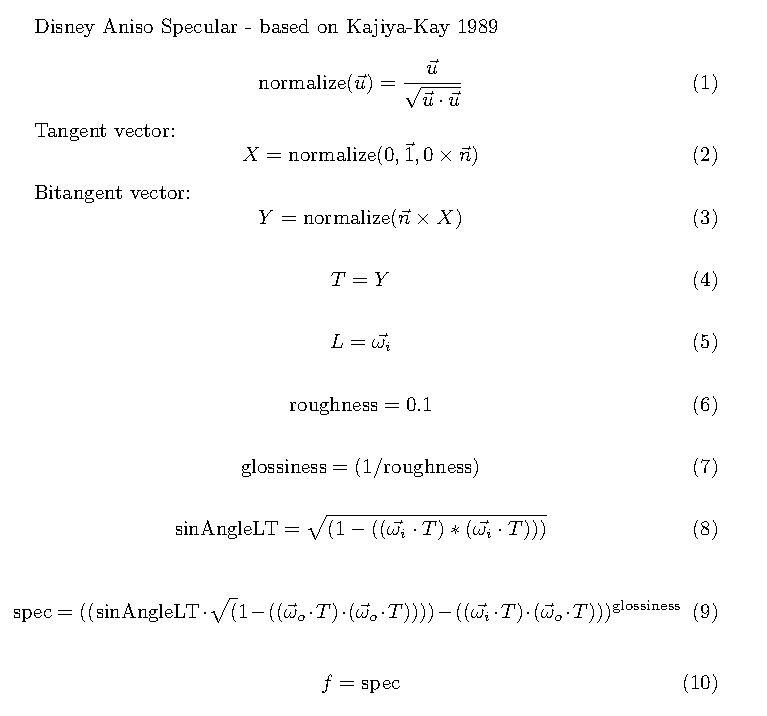
\includegraphics[scale=1.1,width=\textwidth]{./Imagens/brdfs/aniso.pdf}
        
\includegraphics[scale=0.92]{./Imagens/brdfs/blinn-phong.pdf}
    \end{center}
\end{figure}


%%%%%%%%%%%%%%%%%%%%%%%%%%%%%%%%%%%%%%%%%%%%%%%%%
\subsection{Código Fonte em \texttt{EquationLang}}
%%%%%%%%%%%%%%%%%%%%%%%%%%%%%%%%%%%%%%%%%%%%%%%%%
\begin{codigo}[H]
    \caption{\small Código fonte da BRDF do experimento Blinn-Phong.}
    \label{cod-blinn-phong-eqlang}
\begin{lstlisting}[language=tex, frame=none, inputencoding=utf8]
\begin{equation}
    \rho_{d} = \vec{0,1,1}
\end{equation}

\begin{equation}
    \rho_{s} = \vec{1,0,1}
\end{equation}

\begin{equation}
    n = +2^8
\end{equation}

\begin{equation}
f = \frac{\rho_{d}}{\pi} + \rho_{s} * \frac{n+2}{2*\pi} *
\cos{\theta_{h}}^{n}
\end{equation}
\end{lstlisting}
\end{codigo}

%%%%%%%%%%%%%%%%%%%%%%%%%%%%%%%%%%%%%%%%%%%%%%%%%
\subsection{Código GLSL Gerado}
%%%%%%%%%%%%%%%%%%%%%%%%%%%%%%%%%%%%%%%%%%%%%%%%%
\begin{codigo}[H]
    \caption{\small Saída do compilador: código GLSL da BRDF do experimento Blinn-Phong (parte 1 de 2).}
    \label{cod-blinn-phong-glsl-pt-1}
\begin{lstlisting}[language=C, inputencoding=utf8]
analytic ::begin parameters
#[type][name][min val][max val][default val]
::end parameters
::begin shader
//////////// START OF BUILTINS DECLARTION ////////////
vec3 var_0_vec_h;
vec3 var_3_vec_n;
float var_10_theta_h;
float var_11_theta_d;
float var_1_pi;
float var_2_epsilon;
vec3 var_4_vec_omega_i;
float var_5_theta_i;
float var_6_phi_i;
vec3 var_7_vec_omega_o;
float var_8_theta_o;
float var_9_phi_o;
//////////// END OF BUILTINS DECLARTION ////////////
//////////// START OF USER DECLARED ////////////
vec3 var_12_rho_s;
float var_13_n;
vec3 var_14_rho_d;
vec3 var_15_f;
//////////// END OF USER DECLARED ////////////
\end{lstlisting}
\end{codigo}

\begin{codigo}[H]
    \caption{\small Saída do compilador: código GLSL da BRDF do experimento Blinn-Phong (parte 2 de 2).}
    \label{cod-blinn-phong-glsl-pt-2}
\begin{lstlisting}[language=C, inputencoding=utf8]
vec3 BRDF(vec3 L, vec3 V, vec3 N, vec3 X, vec3 Y) {
  //////////// START OF BUILTINS INITIALIZATION ////////////
  var_0_vec_h = normalize(L + V);
  var_3_vec_n = normalize(N);
  var_1_pi = 3.141592653589793;
  var_2_epsilon = 1.192092896e-07;
  var_4_vec_omega_i = L;
  var_5_theta_i = atan(var_4_vec_omega_i.y, var_4_vec_omega_i.x);
  var_6_phi_i = atan(sqrt(var_4_vec_omega_i.y * var_4_vec_omega_i.y +
                          var_4_vec_omega_i.x * var_4_vec_omega_i.x),
                     var_4_vec_omega_i.z);
  var_7_vec_omega_o = V;
  var_8_theta_o = atan(var_7_vec_omega_o.y, var_7_vec_omega_o.x);
  var_9_phi_o = atan(sqrt(var_7_vec_omega_o.y * var_7_vec_omega_o.y +
                          var_7_vec_omega_o.x * var_7_vec_omega_o.x),
                     var_7_vec_omega_o.z);
  var_10_theta_h = acos(dot(var_0_vec_h, N));
  var_11_theta_d = acos(dot(var_0_vec_h, var_4_vec_omega_i));
  //////////// END OF BUILTINS INITIALIZATION ////////////
  var_12_rho_s = vec3(1.0, 0.0, 1.0);
  var_13_n = pow(2.0, 8.0);
  var_14_rho_d = vec3(0.0, 1.0, 1.0);
  var_15_f = ((var_14_rho_d / var_1_pi) +
              ((var_12_rho_s * ((var_13_n + 2.0) / (2.0 * var_1_pi))) *
               pow(cos(var_10_theta_h), var_13_n)));

  return vec3(var_15_f);
}
\end{lstlisting}
\end{codigo}

%%%%%%%%%%%%%%%%%%%%%%%%%%%%%%%%%%%%%%%%%%%%%%%%%
\subsection{Visualização do Resultado}
%%%%%%%%%%%%%%%%%%%%%%%%%%%%%%%%%%%%%%%%%%%%%%%%%

\begin{figure}[H]
  
    \caption{\small{\textit{Plots} da distribuição de reflexão especular e difusa do experimento Blinn-Phong.}}
    \label{fig-blinn-phong-plots}
\minipage{0.48\textwidth}
    \vspace{42px}
  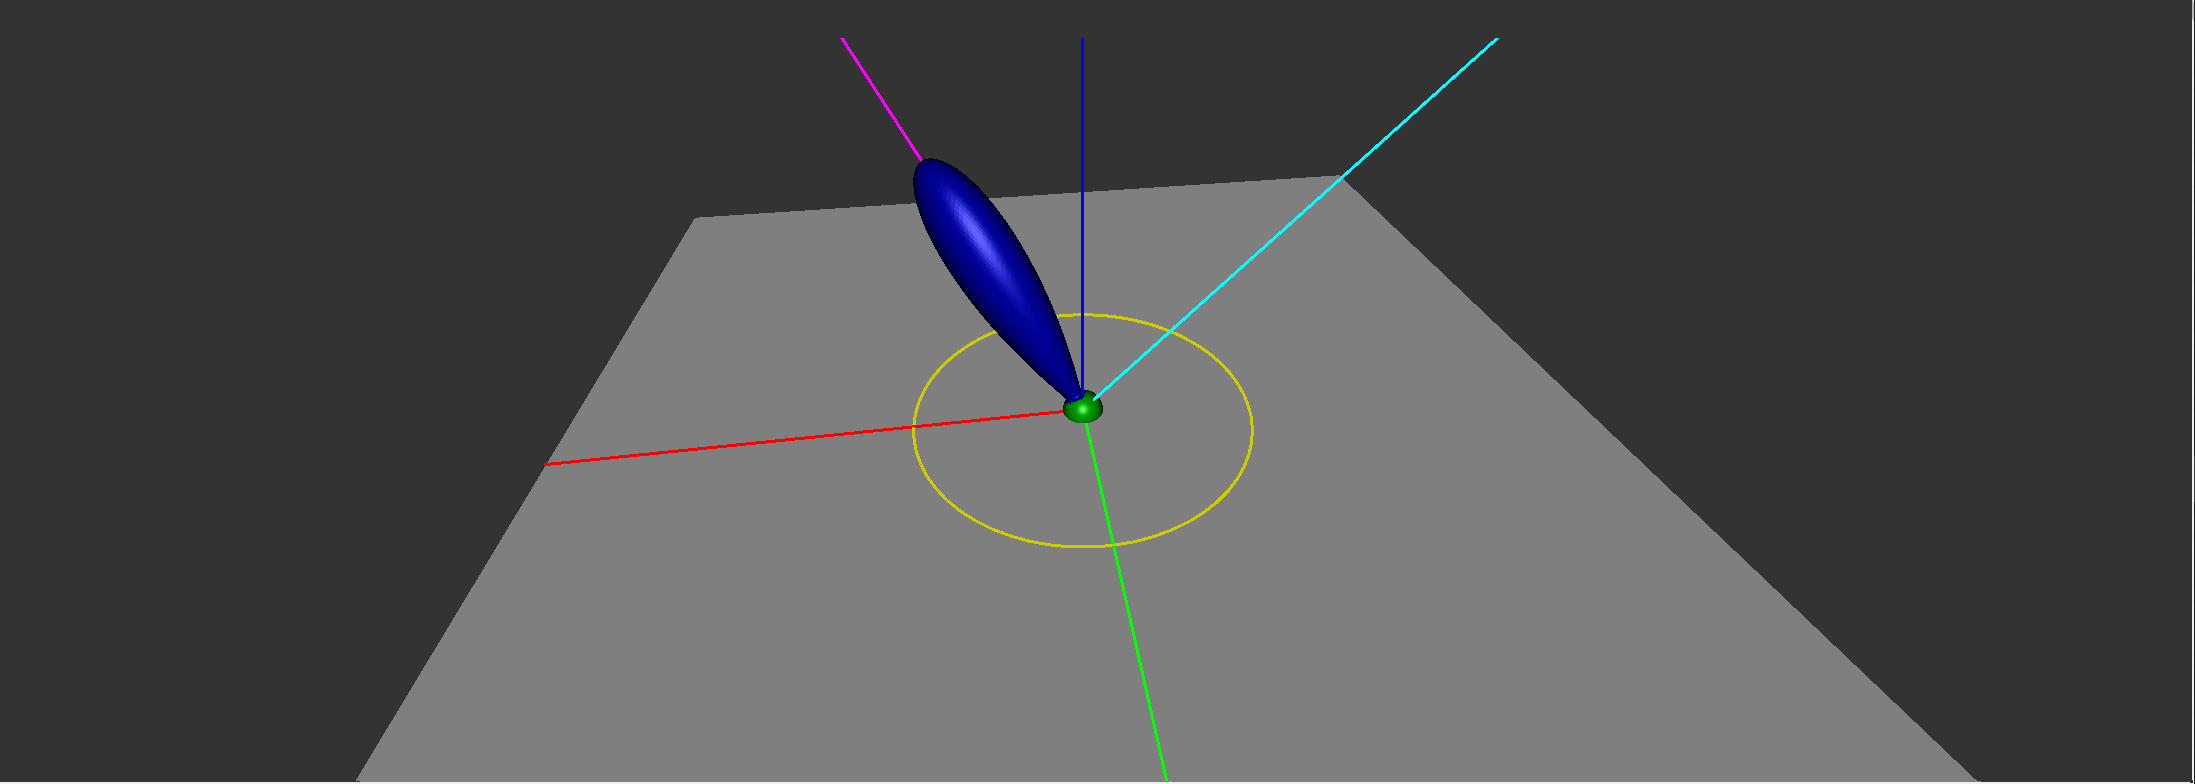
\includegraphics[width=\linewidth]{./Imagens/brdfs/blinn-phong-3D-plot}
    % \caption{\small{(a)}}\label{fig:awesome_image1}
    % \vspace{0.1px}
    \legend{ \small (a) 3D \textit{plot}}
\endminipage\hfill
\minipage{0.48\textwidth}
  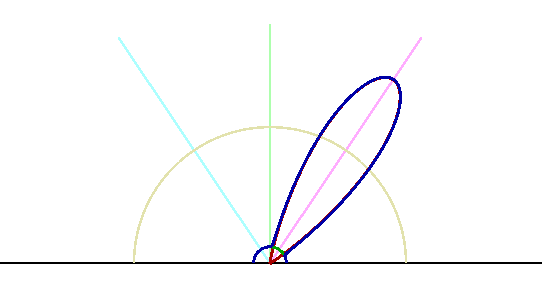
\includegraphics[width=\linewidth]{./Imagens/brdfs/blinn-phong-polar-plot-log.png}
    \legend{ \small (b) \textit{Polar plot}}
    % \caption{\small{(b)}}\label{fig:awesome_image1}
\endminipage\hfill
\end{figure}

\begin{figure}[H]
    \caption{\small{Objetos 3D renderizados pelo experimento Blinn-Phong.}}
    \label{fig-blinn-phong-eqlang}
\minipage{0.32\textwidth}
  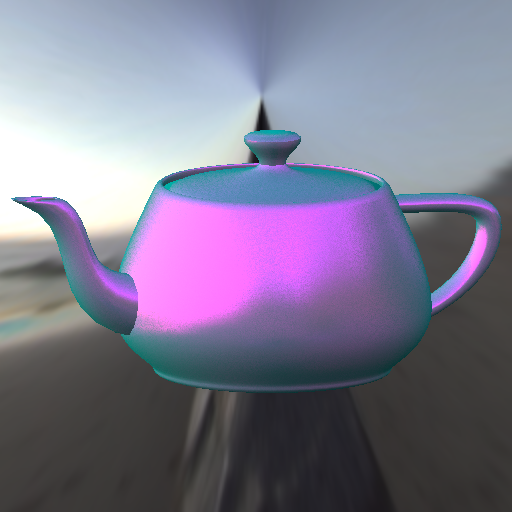
\includegraphics[width=\linewidth]{./Imagens/brdfs/blinn-phong-teapot.png}
    \legend{ \small (a) \textit{Teapot}}
\endminipage\hfill
\minipage{0.32\textwidth}
  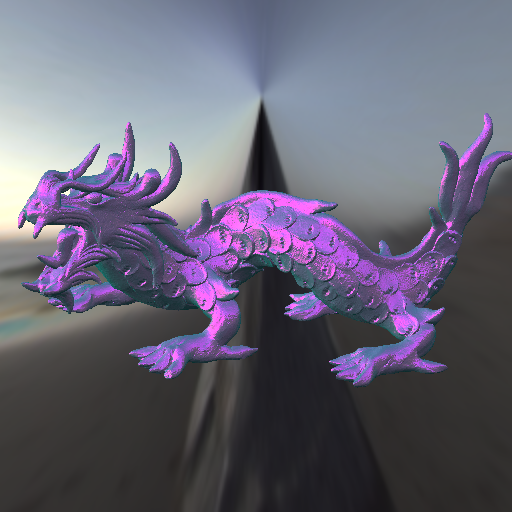
\includegraphics[width=\linewidth]{./Imagens/brdfs/blinn-phong-dragon.png}
    \legend{ \small (b) Dragão de Stanford}
\endminipage\hfill
\minipage{0.32\textwidth}%
  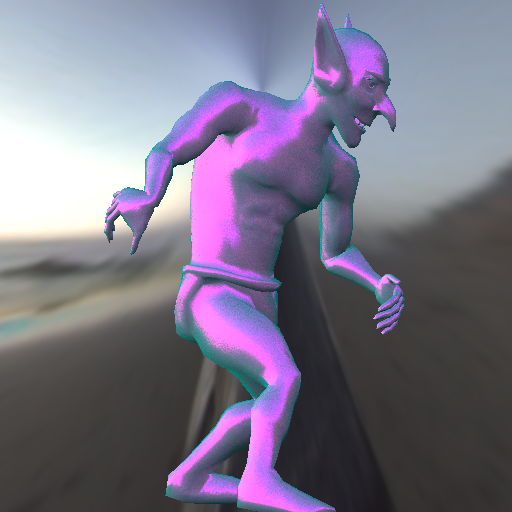
\includegraphics[width=\linewidth]{./Imagens/brdfs/blinn-phong-goblin.png}
    \legend{ \small (c) Goblin}
\endminipage
\end{figure}


\section{Experimento BRDF Cook-Torrance}\label{sec:cook-torrance}

Este experimento é baseada no modelo microfacetado que descreve o comportamento de reflexão de superfícies metálicas descrito no trabalho de Cook-Torrance \cite{cook1982reflectance}. As equações e parametros escolhidos que descrevem esse modelo estão em \autoref{fig-cook-torrance-eqlang-latex}. O código fonte em \texttt{EquationLang} para o compilador está em \autoref{cod-cook-torrance-eqlang}. O código GLSL está dividido em duas partes, parte 1 está no \autoref{cod-cook-torrance-glsl-pt-1} e a segunda parte está em \autoref{cod-cook-torrance-glsl-pt-2}. A renderização dos objetos 3D usando essa BRDF se encontra em \autoref{fig-cook-torrance-eqlang}. Usamos plot logaritmo para gerar os plots 3D e polar presentes na \autoref{fig-cook-torrance-plots}.

%%%%%%%%%%%%%%%%%%%%%%%%%%%%%%%%%%%%%%%%%%%%%%%%%
\subsection{Representação em documento \LaTeX{}}
%%%%%%%%%%%%%%%%%%%%%%%%%%%%%%%%%%%%%%%%%%%%%%%%%
\begin{figure}[H]
    \caption{\label{fig-cook-torrance-eqlang-latex} \small Equações da BRDF do experimento cook-torrance em documento \LaTeX{}.}
    \begin{center}
        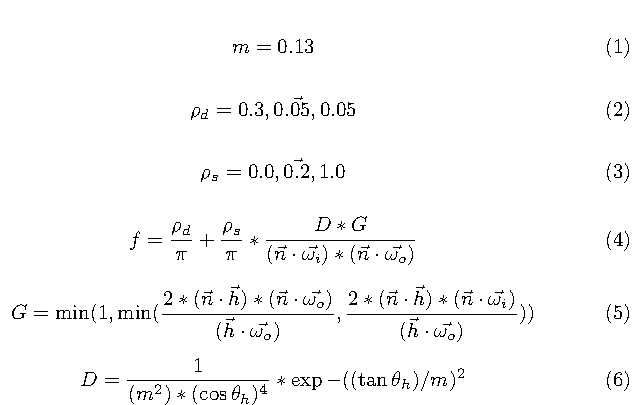
\includegraphics[scale=0.92]{./Imagens/brdfs/cook-torrance.pdf}
    \end{center}
\end{figure}

%%%%%%%%%%%%%%%%%%%%%%%%%%%%%%%%%%%%%%%%%%%%%%%%%
\subsection{Visualização do Resultado}
%%%%%%%%%%%%%%%%%%%%%%%%%%%%%%%%%%%%%%%%%%%%%%%%%
\begin{figure}[H]
    \caption{\small{Distribuição de Reflexão Especular e Difusa da BRDF}}\label{fig-cook-torrance-plots}
\minipage{0.48\textwidth}
    \vspace{42px}
  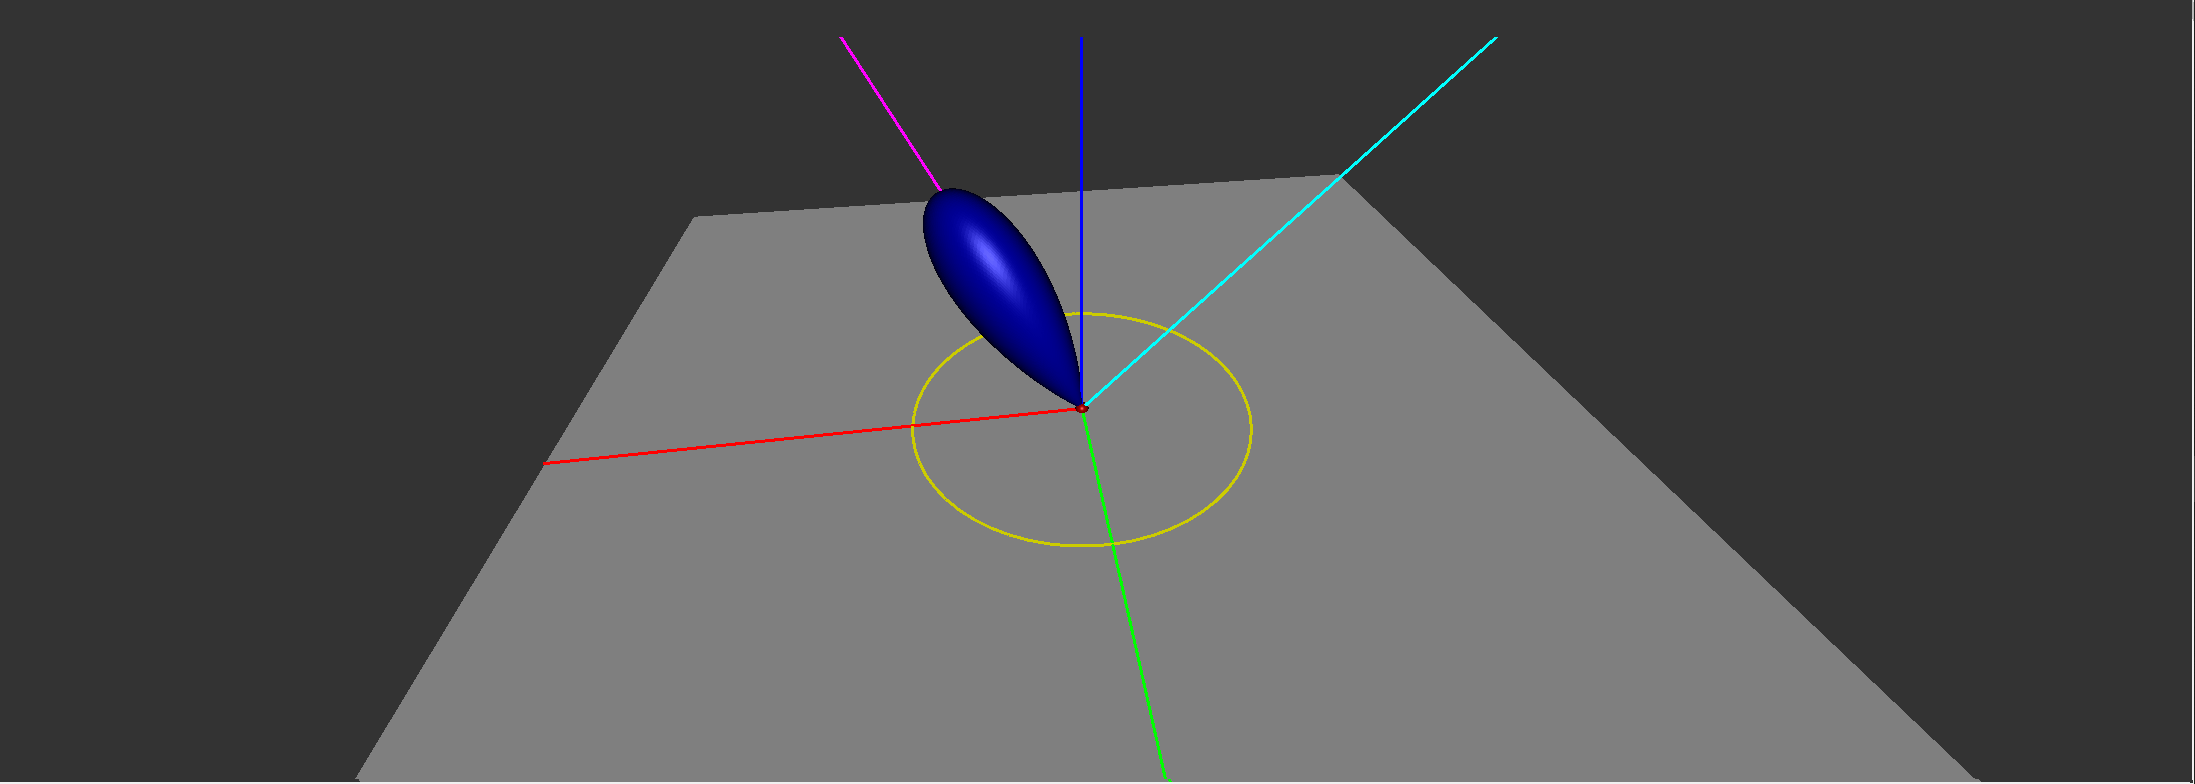
\includegraphics[width=\linewidth]{./Imagens/brdfs/cook-torrance-3D-plot}
    % \vspace{0.1px}
    \legend{ \small (a) 3D \textit{plot}}
\endminipage\hfill
\minipage{0.48\textwidth}
  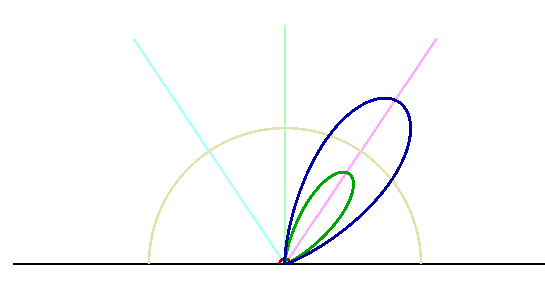
\includegraphics[width=\linewidth]{./Imagens/brdfs/cook-torrance-polar-plot-log.png}
    \legend{ \small (b) \textit{Polar plot}}
\endminipage\hfill
\end{figure}

\begin{figure}[H]
    \caption{\small{Objetos 3D renderizados por este experimento}}\label{fig-cook-torrance-eqlang}
\minipage{0.32\textwidth}
  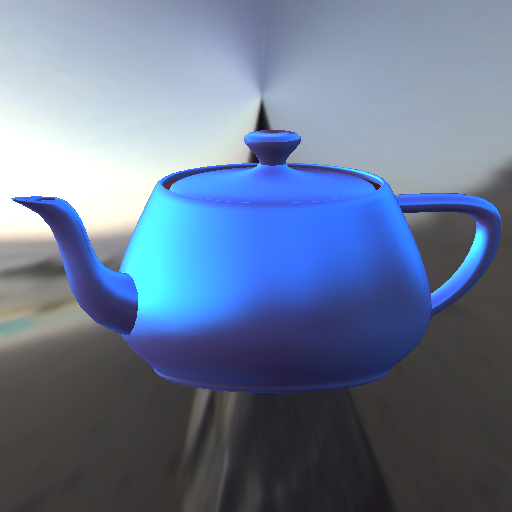
\includegraphics[width=\linewidth]{./Imagens/brdfs/cook-torrance-teapot.png}
    \legend{ \small (a) \textit{Teapot}}
\endminipage\hfill
\minipage{0.32\textwidth}
  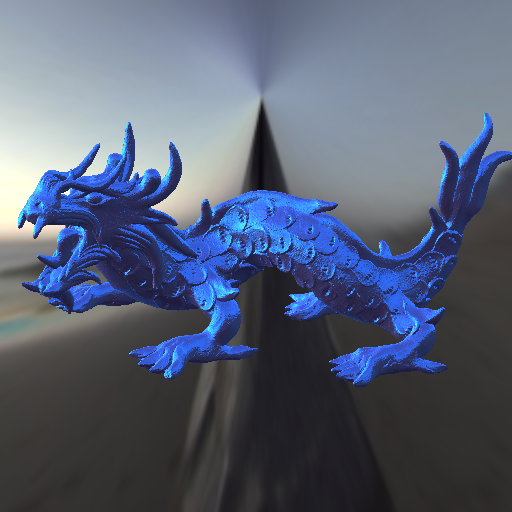
\includegraphics[width=\linewidth]{./Imagens/brdfs/cook-torrance-dragon.png}
    \legend{ \small (b) Dragão de Stanford}
\endminipage\hfill
\minipage{0.32\textwidth}%
  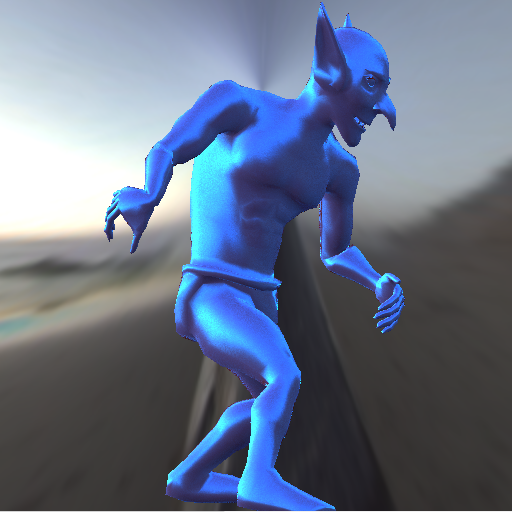
\includegraphics[width=\linewidth]{./Imagens/brdfs/cook-torrance-goblin.png}
    \legend{ \small (c) Goblin}
\endminipage
\end{figure}

%%%%%%%%%%%%%%%%%%%%%%%%%%%%%%%%%%%%%%%%%%%%%%%%%
\subsection{Código GLSL Gerado}
%%%%%%%%%%%%%%%%%%%%%%%%%%%%%%%%%%%%%%%%%%%%%%%%%
\begin{codigo}[H]
    \caption{\small Saida do compilador, código GLSL da BRDF deste experimento (parte 1). }
    \label{cod-cook-torrance-glsl-pt-1}
\begin{lstlisting}[language=C, inputencoding=utf8]
analytic ::begin parameters
#[type][name][min val][max val][default val]
::end parameters
::begin shader
//////////// START OF BUILTINS DECLARTION ////////////
vec3 var_0_vec_h;
vec3 var_3_vec_n;
float var_10_theta_h;
float var_11_theta_d;
float var_1_pi;
float var_2_epsilon;
vec3 var_4_vec_omega_i;
float var_5_theta_i;
float var_6_phi_i;
vec3 var_7_vec_omega_o;
float var_8_theta_o;
float var_9_phi_o;
//////////// END OF BUILTINS DECLARTION ////////////
//////////// START OF USER DECLARED ////////////
float var_12_G;
vec3 var_13_rho_s;
float var_14_m;
float var_15_D;
vec3 var_16_rho_d;
vec3 var_17_f;
//////////// END OF USER DECLARED ////////////
//////////// START FUNCTIONS DECLARATIONS ////////////
//////////// END FUNCTIONS DECLARATIONS ////////////
\end{lstlisting}
\end{codigo}

\begin{codigo}[H]
    \caption{\small Saida do compilador, código GLSL da BRDF deste experimento  (parte 2). }
    \label{cod-cook-torrance-glsl-pt-2}
\begin{lstlisting}[language=C, inputencoding=utf8]
vec3 BRDF(vec3 L, vec3 V, vec3 N, vec3 X, vec3 Y) {

  //////////// START OF BUILTINS INITIALIZATION ////////////
  var_0_vec_h = normalize(L + V);
  var_3_vec_n = normalize(N);
  var_1_pi = 3.141592653589793;
  var_2_epsilon = 1.192092896e-07;
  var_4_vec_omega_i = L;
  var_5_theta_i = atan(var_4_vec_omega_i.y, var_4_vec_omega_i.x);
  var_6_phi_i = atan(sqrt(var_4_vec_omega_i.y * var_4_vec_omega_i.y +
                          var_4_vec_omega_i.x * var_4_vec_omega_i.x),
                     var_4_vec_omega_i.z);
  var_7_vec_omega_o = V;
  var_8_theta_o = atan(var_7_vec_omega_o.y, var_7_vec_omega_o.x);
  var_9_phi_o = atan(sqrt(var_7_vec_omega_o.y * var_7_vec_omega_o.y +
                          var_7_vec_omega_o.x * var_7_vec_omega_o.x),
                     var_7_vec_omega_o.z);
  var_10_theta_h = acos(dot(var_0_vec_h, N));
  var_11_theta_d = acos(dot(var_0_vec_h, var_4_vec_omega_i));
  //////////// END OF BUILTINS INITIALIZATION ////////////

  var_12_G = min(1.0, min((((2.0 * (dot(var_3_vec_n, var_0_vec_h))) *
                            (dot(var_3_vec_n, var_7_vec_omega_o))) /
                           (dot(var_0_vec_h, var_7_vec_omega_o))),
                          (((2.0 * (dot(var_3_vec_n, var_0_vec_h))) *
                            (dot(var_3_vec_n, var_4_vec_omega_i))) /
                           (dot(var_0_vec_h, var_7_vec_omega_o)))));
  var_13_rho_s = vec3(0.0, 0.2, 1.0);
  var_14_m = 0.13;
  var_15_D = ((1.0 / ((pow(var_14_m, 2.0)) * pow((cos(var_10_theta_h)), 4.0))) *
              exp((-pow((((tan(var_10_theta_h)) / var_14_m)), 2.0))));
  var_16_rho_d = vec3(0.3, 0.05, 0.05);
  var_17_f =
      ((var_16_rho_d / var_1_pi) +
       ((var_13_rho_s / var_1_pi) *
        ((var_15_D * var_12_G) / ((dot(var_3_vec_n, var_4_vec_omega_i)) *
                                  (dot(var_3_vec_n, var_7_vec_omega_o))))));

  return vec3(var_17_f);
}
\end{lstlisting}
\end{codigo}

%%%%%%%%%%%%%%%%%%%%%%%%%%%%%%%%%%%%%%%%%%%%%%%%%
\subsection{Código Fonte em \texttt{EquationLang}}
%%%%%%%%%%%%%%%%%%%%%%%%%%%%%%%%%%%%%%%%%%%%%%%%%
\begin{codigo}[H]
    \caption{\small Código fonte da BRDF deste experimento.}
    \label{cod-cook-torrance-eqlang}
\begin{lstlisting}[language=tex, frame=none, inputencoding=utf8]
\begin{equation}
m = 0.13
\end{equation}

\begin{equation}
    \rho_{d} = \vec{0.3,0.05,0.05}
\end{equation}

\begin{equation}
    \rho_{s} = \vec{0.0,0.2,1.0}
\end{equation}

\begin{equation}
f = \frac{\rho_{d}}{\pi} +
\frac{\rho_{s}}{\pi} *
\frac{D*G}{({\vec{n}}\cdot{\vec{\omega_{i}}}) *
({\vec{n}}\cdot{\vec{\omega_{o}}})}
\end{equation}

\begin{equation}
G = \min(1,\min(
\frac{2 *
({\vec{n}}\cdot{\vec{h}}) *
({\vec{n}}\cdot{\vec{\omega_{o}}})
}
{({\vec{h}}\cdot{\vec{\omega_{o}}})},
\frac{2 *
({\vec{n}}\cdot{\vec{h}}) *
({\vec{n}}\cdot{\vec{\omega_{i}}})
}
{({\vec{h}}\cdot{\vec{\omega_{o}}})}
))
\end{equation}

\begin{equation}
D = \frac{1}
{(m^{2}) * (\cos{\theta_{h}})^{4}} *
\exp{-((\tan{\theta_{h}})/m)^{2}}
\end{equation}
\end{lstlisting}
\end{codigo}


\section{Experimento BRDF Ward} \label{section-experiment-ward}

Este experimento é baseado na BRDF revisada segundo as notas de Walter \cite{walter2005notes}, que detalham o modelo de Ward. Suas equações podem ser vistas na \autoref{fig-ward-eqlang-latex}, enquanto o código em \texttt{EquationLang} está disponível no \autoref{cod-ward-eqlang-pt-1} (parte 1) e no \autoref{cod-ward-eqlang-pt-2} (parte 2). O código gerado pelo compilador é formado pelo \autoref{cod-ward-glsl-pt-1} e pelo \autoref{cod-ward-glsl-pt-2}. A renderização de objetos usando este modelo é ilustrada na \autoref{fig-ward-objetcs}, e os \textit{plots} da sua refletância estão na \autoref{fig-ward-plots}.
%%


%%%%%%%%%%%%%%%%%%%%%%%%%%%%%%%%%%%%%%%%%%%%%%%%%
\subsection{Representação em documento \LaTeX{}}
%%%%%%%%%%%%%%%%%%%%%%%%%%%%%%%%%%%%%%%%%%%%%%%%%
\begin{figure}[H]
    \caption{\label{fig-ward-eqlang-latex} \small Equações da BRDF do experimento Ward em documento \LaTeX{}.}
    \begin{center}
        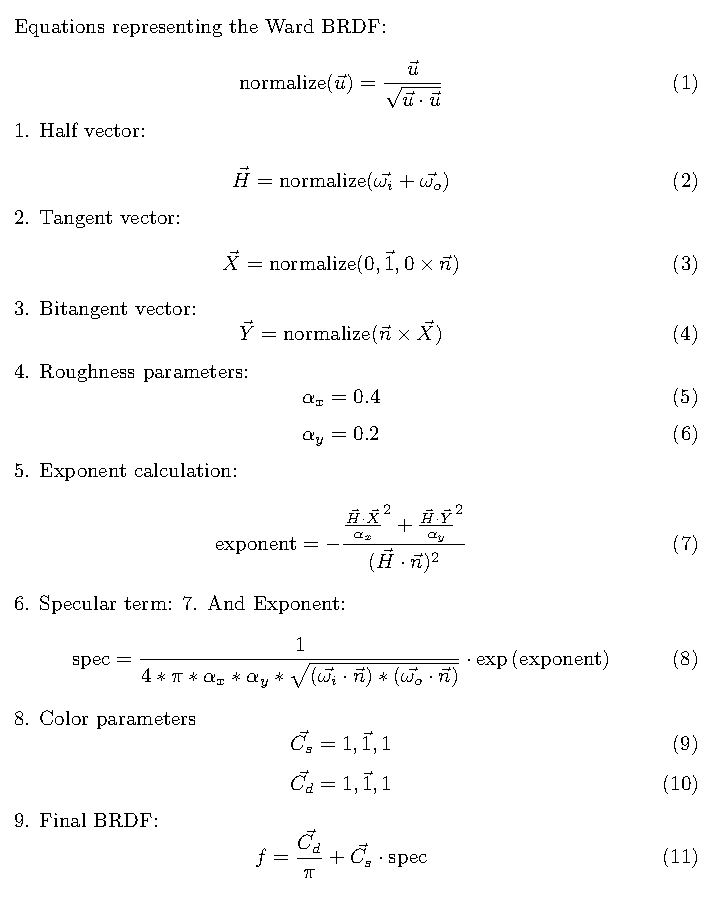
\includegraphics[scale=0.92]{./Imagens/brdfs/ward.pdf}
    \end{center}
\end{figure}

%%%%%%%%%%%%%%%%%%%%%%%%%%%%%%%%%%%%%%%%%%%%%%%%%
\subsection{Código Fonte em \texttt{EquationLang}}
%%%%%%%%%%%%%%%%%%%%%%%%%%%%%%%%%%%%%%%%%%%%%%%%%
\begin{codigo}[H]
    \caption{\small Código fonte da BRDF do experimento Ward (parte 1 de 2).}
    \label{cod-ward-eqlang-pt-1}
\begin{lstlisting}[language=tex, frame=none, inputencoding=utf8]
Equations representing the Ward BRDF:
   \begin{equation}
      \text{normalize}(\vec{u}) = \frac{\vec{u}}{\sqrt{\vec{u} \cdot \vec{u}}}
   \end{equation}
1. Half vector:
   \begin{equation}
   \vec{H} = \text{normalize}(\vec{\omega_i} + \vec{\omega_o})
   \end{equation}
2. Tangent vector:
   \begin{equation}
   \vec{X} = \text{normalize}(\vec{0,1,0} \times \vec{n})
   \end{equation}
3. Bitangent vector:
   \begin{equation}
   \vec{Y} = \text{normalize}(\vec{n} \times \vec{X})
   \end{equation}
4. Roughness parameters:
   \begin{equation}
   \alpha_x = 0.4
   \end{equation}
   \begin{equation}
   \alpha_y = 0.2
   \end{equation}
\end{lstlisting}
\end{codigo}

\begin{codigo}[H]
    \caption{\small Código fonte da BRDF do experimento Ward (parte 2 de 2).}
    \label{cod-ward-eqlang-pt-2}
\begin{lstlisting}[language=tex, frame=none, inputencoding=utf8]
5. Exponent calculation:
   \begin{equation}
   \text{exponent} = -\frac{
       \frac{\vec{H} \cdot \vec{X}}{\alpha_x}^2 +
       \frac{\vec{H} \cdot \vec{Y}}{\alpha_y}^2
   }{(\vec{H} \cdot \vec{n})^2}
   \end{equation}
6. Specular term:
7. And Exponent:
   \begin{equation}
   \text{spec} = \frac{1}{4*\pi * \alpha_x *\alpha_y *\sqrt{(\vec{\omega_i} \cdot \vec{n}) * (\vec{\omega_o} \cdot \vec{n})}}
      \cdot \exp{( \text{exponent} )}
   \end{equation}
8. Color parameters
   \begin{equation}
   \vec{C_s} = \vec{1, 1, 1}
   \end{equation}
   \begin{equation}
   \vec{C_d} = \vec{ 1, 1, 1 }
   \end{equation}
9. Final BRDF:
   \begin{equation}
   f = \frac{\vec{C_d}}{\pi} + \vec{C_s} \cdot \text{spec}
   \end{equation}
\end{lstlisting}
\end{codigo}

%%%%%%%%%%%%%%%%%%%%%%%%%%%%%%%%%%%%%%%%%%%%%%%%%
\subsection{Código GLSL Gerado}
%%%%%%%%%%%%%%%%%%%%%%%%%%%%%%%%%%%%%%%%%%%%%%%%%
\begin{codigo}[H]
    \caption{\small Saída do compilador: código GLSL da BRDF do experimento Ward (parte 1 de 2).}
    \label{cod-ward-glsl-pt-1}
\begin{lstlisting}[language=C, inputencoding=utf8]
analytic
::begin parameters
#[type][name][min val][max val][default val]
::end parameters
::begin shader
//////////// START OF BUILTINS DECLARTION ////////////
vec3 var_0_vec_h;
vec3 var_3_vec_n;
float var_10_theta_h;
float var_11_theta_d;
float var_1_pi;
float var_2_epsilon;
vec3 var_4_vec_omega_i;
float var_5_theta_i;
float var_6_phi_i;
vec3 var_7_vec_omega_o;
float var_8_theta_o;
float var_9_phi_o;
//////////// END OF BUILTINS DECLARTION ////////////
//////////// START OF USER DECLARED ////////////
vec3 var_14_vec_X;
vec3 var_15_vec_Y;
float var_16_alpha_x;
float var_17_alpha_y;
vec3 var_18_vec_C_d;
vec3 var_19_vec_C_s;
vec3 var_20_vec_H;
float var_21_text_exponent;
float var_22_text_spec;
vec3 var_23_f;
//////////// END OF USER DECLARED ////////////
//////////// START FUNCTIONS DECLARATIONS ////////////
vec3 var_12_text_normalize(vec3 var_13_vec_u) {
  return (var_13_vec_u / sqrt(dot(var_13_vec_u, var_13_vec_u)));
}
//////////// END FUNCTIONS DECLARATIONS ////////////
\end{lstlisting}
\end{codigo}

\begin{codigo}[H]
    \caption{\small Saída do compilador: código GLSL da BRDF do experimento Ward (parte 2 de 2).}
\label{cod-ward-glsl-pt-2}
\begin{lstlisting}[language=C, inputencoding=utf8]
vec3 BRDF(vec3 L, vec3 V, vec3 N, vec3 X, vec3 Y) {
  //////////// START OF BUILTINS INITIALIZATION ////////////
  var_0_vec_h = normalize(L + V);
  var_3_vec_n = normalize(N);
  var_1_pi = 3.141592653589793;
  var_2_epsilon = 1.192092896e-07;
  var_4_vec_omega_i = L;
  var_5_theta_i = atan(var_4_vec_omega_i.y, var_4_vec_omega_i.x);
  var_6_phi_i = atan(sqrt(var_4_vec_omega_i.y * var_4_vec_omega_i.y +
                          var_4_vec_omega_i.x * var_4_vec_omega_i.x),
                     var_4_vec_omega_i.z);
  var_7_vec_omega_o = V;
  var_8_theta_o = atan(var_7_vec_omega_o.y, var_7_vec_omega_o.x);
  var_9_phi_o = atan(sqrt(var_7_vec_omega_o.y * var_7_vec_omega_o.y +
                          var_7_vec_omega_o.x * var_7_vec_omega_o.x),
                     var_7_vec_omega_o.z);
  var_10_theta_h = acos(dot(var_0_vec_h, N));
  var_11_theta_d = acos(dot(var_0_vec_h, var_4_vec_omega_i));
  //////////// END OF BUILTINS INITIALIZATION ////////////
  var_14_vec_X = var_12_text_normalize(cross(vec3(0.0, 1.0, 0.0), var_3_vec_n));
  var_15_vec_Y = var_12_text_normalize(cross(var_3_vec_n, var_14_vec_X));
  var_16_alpha_x = 0.4;
  var_17_alpha_y = 0.2;
  var_18_vec_C_d = vec3(1.0, 1.0, 1.0);
  var_19_vec_C_s = vec3(1.0, 1.0, 1.0);
  var_20_vec_H = var_12_text_normalize((var_4_vec_omega_i + var_7_vec_omega_o));
  var_21_text_exponent = (-((pow((dot(var_20_vec_H, var_14_vec_X) / var_16_alpha_x), 2.0) +
          pow((dot(var_20_vec_H, var_15_vec_Y) / var_17_alpha_y), 2.0)) /
         pow((dot(var_20_vec_H, var_3_vec_n)), 2.0)));
  var_22_text_spec = ((1.0 / ((((4.0 * var_1_pi) * var_16_alpha_x) * var_17_alpha_y) *
               sqrt(((dot(var_4_vec_omega_i, var_3_vec_n)) *
                     (dot(var_7_vec_omega_o, var_3_vec_n)))))) *
       exp((var_21_text_exponent)));
  var_23_f = ((var_18_vec_C_d / var_1_pi) + (var_19_vec_C_s * var_22_text_spec));

  return vec3(var_23_f);
}
\end{lstlisting}
\end{codigo}

%%%%%%%%%%%%%%%%%%%%%%%%%%%%%%%%%%%%%%%%%%%%%%%%%
\subsection{Visualização do Resultado}
%%%%%%%%%%%%%%%%%%%%%%%%%%%%%%%%%%%%%%%%%%%%%%%%%
\begin{figure}[H]
    \caption{\small{\textit{Plots} da distribuição de reflexão especular e difusa do experimento Ward.}}
    \label{fig-ward-plots}

\minipage{0.48\textwidth}
    \vspace{42px}
  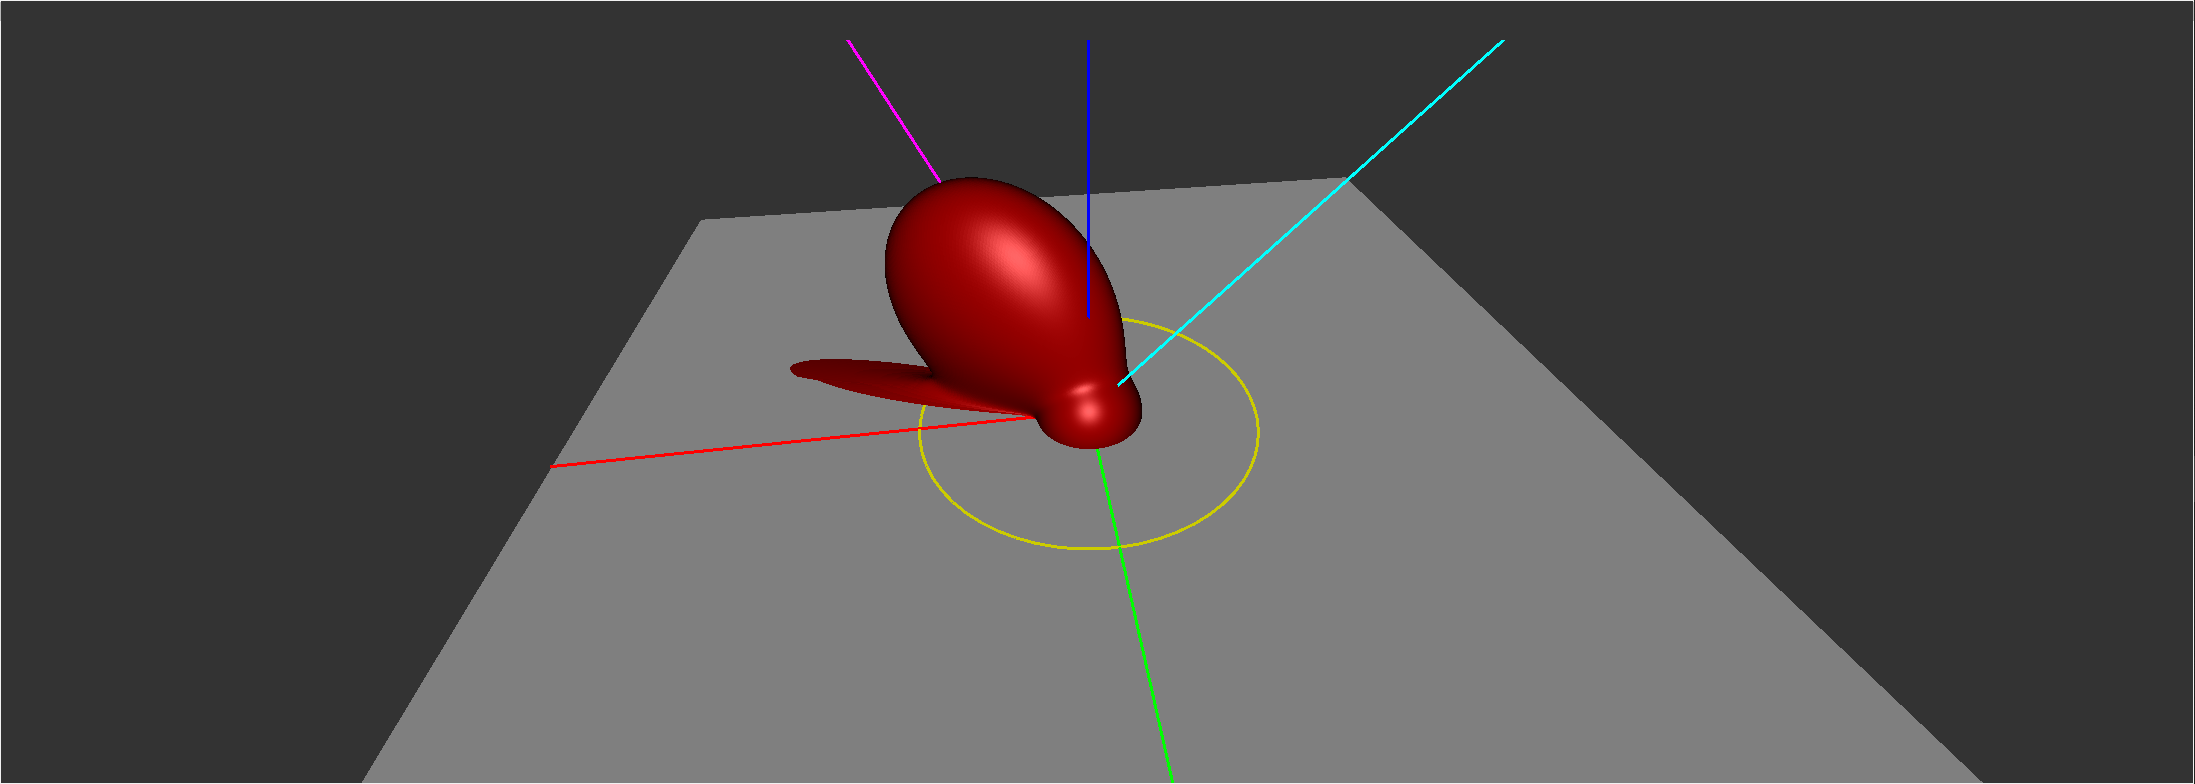
\includegraphics[width=\linewidth]{./Imagens/brdfs/ward-3D-plot}
    % \vspace{0.1px}
    \legend{ \small (a) 3D \textit{plot}}
\endminipage\hfill
\minipage{0.48\textwidth}
  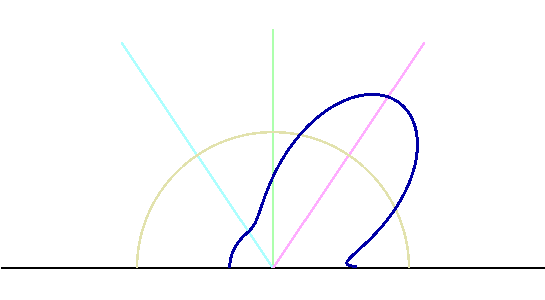
\includegraphics[width=\linewidth]{./Imagens/brdfs/ward-polar-plot.png}
    \legend{ \small (b) \textit{Polar plot}}
\endminipage\hfill
\end{figure}

\begin{figure}[H]
    \caption{\small{Objetos 3D renderizados pelo experimento Ward.}}\label{fig-ward-objetcs}
\minipage{0.32\textwidth}
  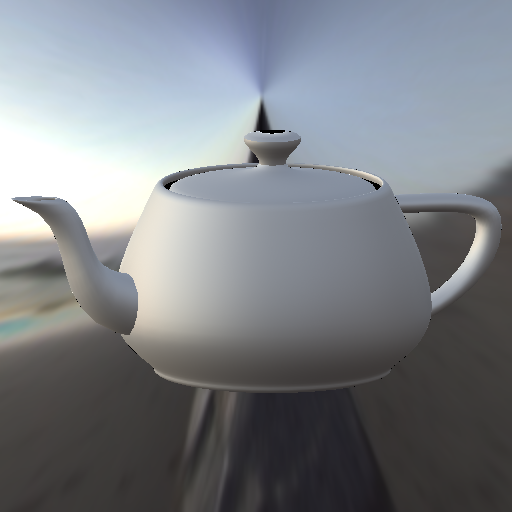
\includegraphics[width=\linewidth]{./Imagens/brdfs/ward-teapot.png}
    \legend{ \small (a) \textit{Teapot}}
\endminipage\hfill
\minipage{0.32\textwidth}
  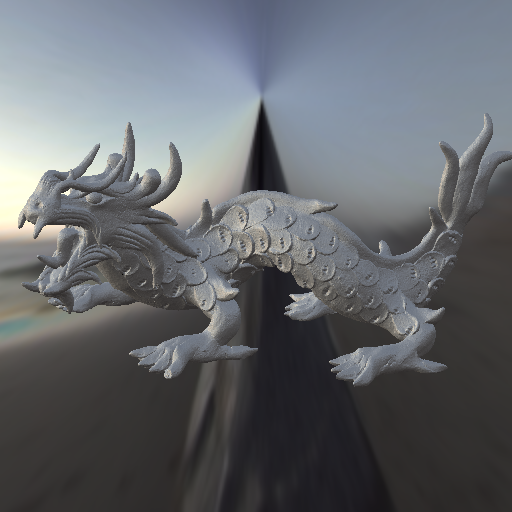
\includegraphics[width=\linewidth]{./Imagens/brdfs/ward-dragon.png}
    \legend{ \small (b) Dragão de Stanford}
\endminipage\hfill
\minipage{0.32\textwidth}%
  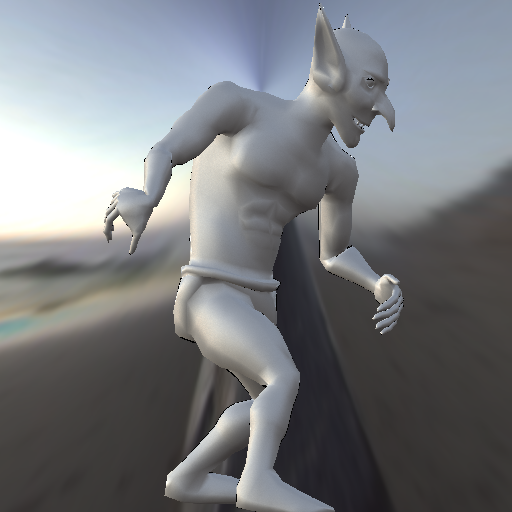
\includegraphics[width=\linewidth]{./Imagens/brdfs/ward-goblin.png}
    \legend{ \small (c) Goblin}
\endminipage
\end{figure}



\section{Experimento BRDF Ashikhmin-Shirley}\label{sec:ashikhmin-shirley}

Neste experimento, utilizamos uma BRDF anisotrópica desenvolvida por Ashikhmin-Shirley \cite{ashikhmin2000anisotropic}, que apresenta um modelo de reflexão não uniforme. A descrição matemática está presente na \autoref{fig-ashikhmin-shirley-close-to-original-eqlang-latex}, com o código-fonte em \texttt{EquationLang} disponível no \autoref{cod-ashikhmin-shirley-close-to-original-eqlang-pt-1} e no \autoref{cod-ashikhmin-shirley-close-to-original-eqlang-pt-2}. Destacamos que o compilador corretamente ignora texto fora do ambiente \texttt{equation}. O código gerado em GLSL é apresentado no \autoref{cod-ashikhmin-shirley-close-to-original-glsl-pt-1} e no \autoref{cod-ashikhmin-shirley-close-to-original-glsl-pt-2}. A renderização dos objetos 3D pode ser observada na \autoref{fig-ashikhmin-shirley-close-to-original-eqlang}, e os \textit{plots} correspondentes estão na \autoref{fig-ashikhmin-shirley-close-to-original-plots}.
%

%%%%%%%%%%%%%%%%%%%%%%%%%%%%%%%%%%%%%%%%%%%%%%%%%
\subsection{Representação em documento \LaTeX{}}
%%%%%%%%%%%%%%%%%%%%%%%%%%%%%%%%%%%%%%%%%%%%%%%%%
\begin{figure}[H]
    \caption{\label{fig-ashikhmin-shirley-close-to-original-eqlang-latex}
    \small Equações da BRDF do experimento Ashikhmin-Shirley em documento \LaTeX{}.}
    \begin{center}
        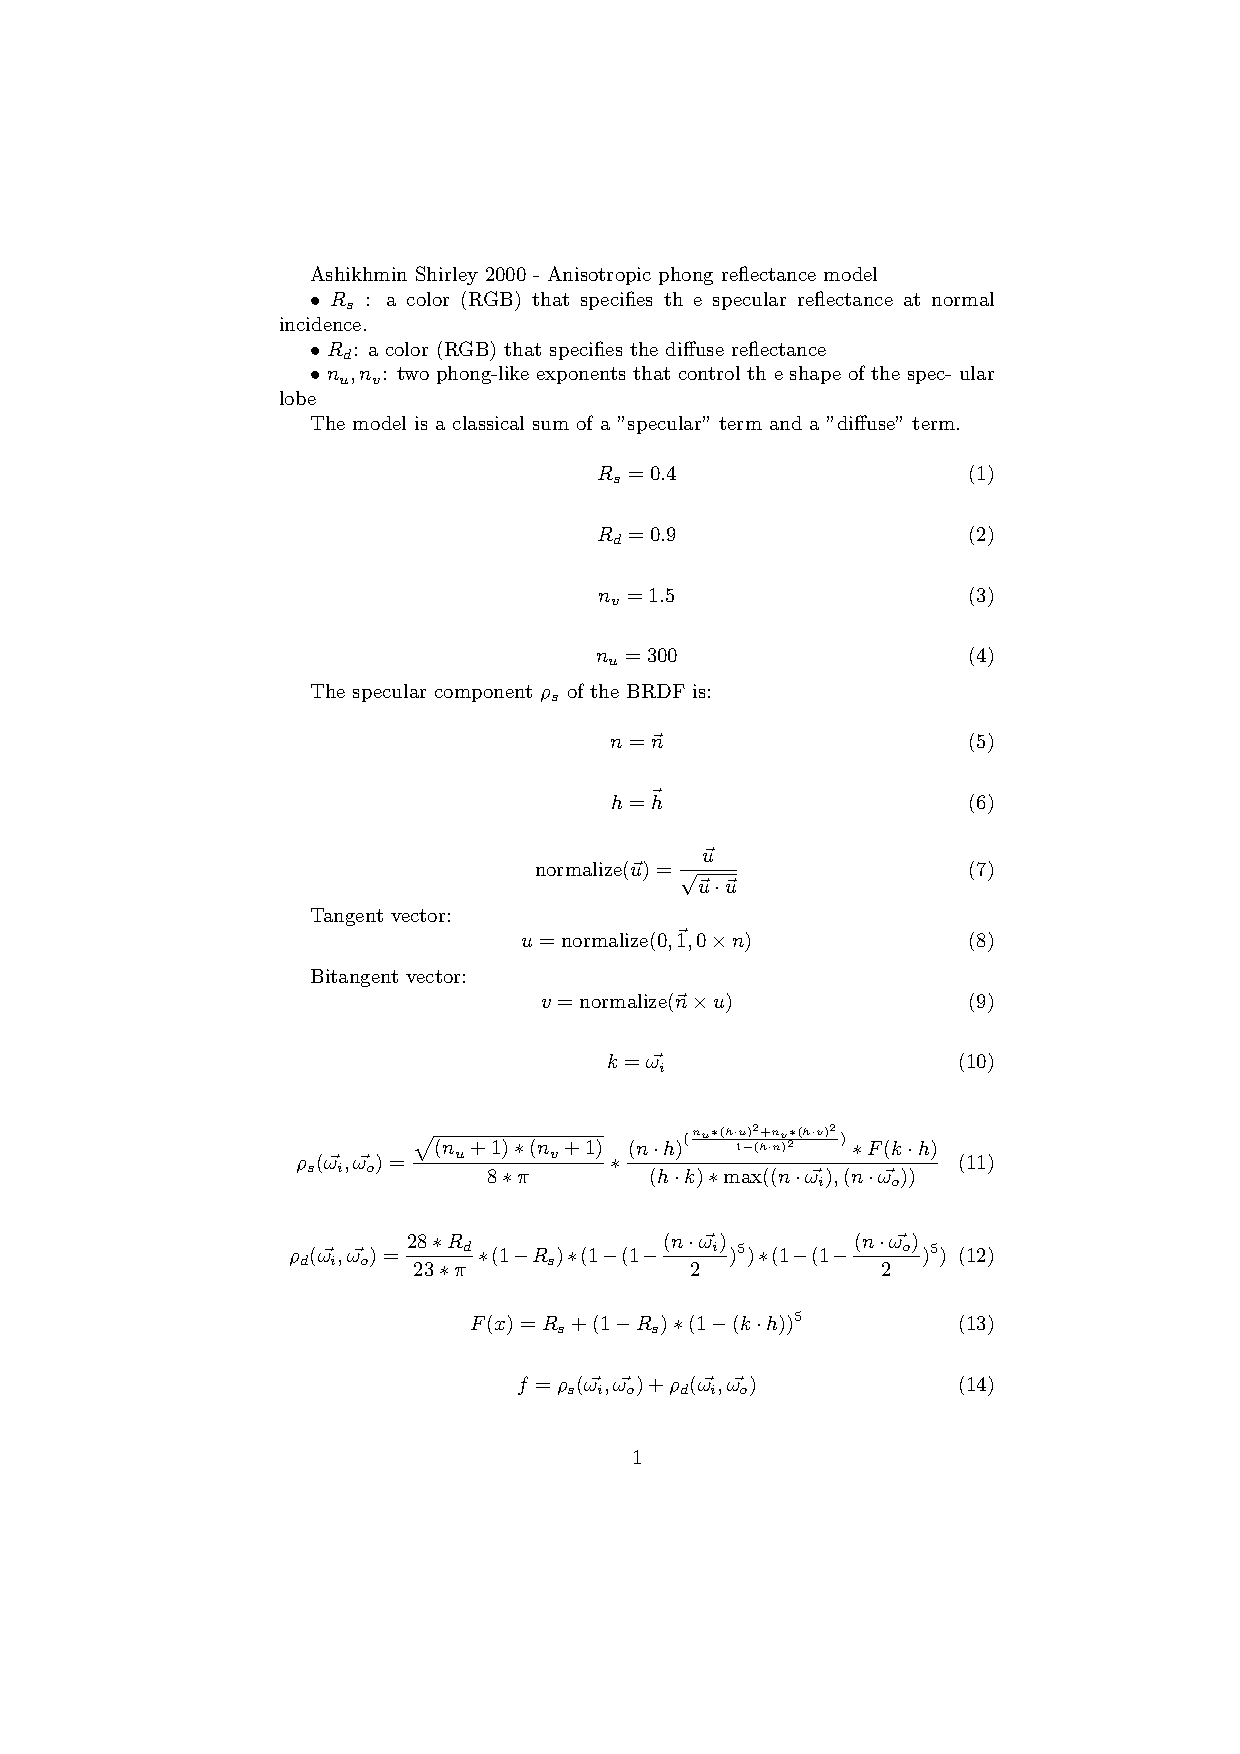
\includegraphics[scale=0.92]{./Imagens/brdfs/ashikhmin-shirley-close-to-original.pdf}
    \end{center}
\end{figure}


%%%%%%%%%%%%%%%%%%%%%%%%%%%%%%%%%%%%%%%%%%%%%%%%%
\subsection{Código Fonte em \texttt{EquationLang}}
%%%%%%%%%%%%%%%%%%%%%%%%%%%%%%%%%%%%%%%%%%%%%%%%%
\begin{codigo}[H]
    \caption{\small Código fonte da BRDF do experimento Ashikhmin-Shirley (parte 1 de 2).}
    \label{cod-ashikhmin-shirley-close-to-original-eqlang-pt-1}
\begin{lstlisting}[language=tex, frame=none, inputencoding=utf8]
Ashikhmin Shirley 2000 - Anisotropic phong reflectance model

 $R_s$ : a color (RGB) that specifies th e specular reflectance
at normal incidence.

 $R_d$: a color (RGB) that specifies the diffuse reflectance

 $n_u, n_v$: two phong-like exponents that control th e shape of the spec- ular lobe

The model is a classical sum of a "specular" term and a "diffuse" term.

\begin{equation}
    R_s = 0.4
\end{equation}

\begin{equation}
    R_d = 0.9
\end{equation}

\begin{equation}
    n_v = 1.5
\end{equation}

\begin{equation}
    n_u = 300
\end{equation}

The specular component $\rho_s$ of the BRDF is:

\begin{equation}
    n = \vec n
\end{equation}

\begin{equation}
    h = \vec h
\end{equation}
\end{equation}
\end{lstlisting}
\end{codigo}



\begin{codigo}[H]
    \caption{\small Código fonte da BRDF do experimento Ashikhmin-Shirley (parte 2 de 2).}
    \label{cod-ashikhmin-shirley-close-to-original-eqlang-pt-2}
\begin{lstlisting}[language=tex, frame=none, inputencoding=utf8]
\begin{equation}
  \text{normalize}(\vec{u}) = \frac{\vec{u}}{\sqrt{\vec{u} \cdot \vec{u}}}
\end{equation}
Tangent vector:
\begin{equation}
   u = \text{normalize}(\vec{0,1,0} \times n)
Bitangent vector:
\begin{equation}
   v = \text{normalize}(\vec{n} \times u)
\end{equation}

\begin{equation}
    k = \vec{\omega_i}
\end{equation}

\begin{equation}
    \rho_s(\vec{\omega_i}, \vec{\omega_o}) =
        \frac{\sqrt{(n_u+1)*(n_v+1)}}{8*\pi}
        * \frac{(n \cdot h)^{(\frac{n_u * (h \cdot u )^2 + n_v *(h \cdot v)^2}{1-(h \cdot n)^2})}
        * F(k \cdot h)}{(h \cdot k) * \max((n \cdot \vec{\omega_i}), (n \cdot \vec{\omega_o}) )}
\end{equation}

\begin{equation}
    \rho_d(\vec{\omega_i}, \vec{\omega_o}) = \frac{28*R_d}{23*\pi}
        * (1-R_s)
        * (1-(1-\frac{(n \cdot \vec{\omega_i})}{2})^5)
        * (1-(1-\frac{(n \cdot \vec{\omega_o})}{2})^5)
\end{equation}

\begin{equation}
    F(x) = R_s + (1-R_s)*(1-(k \cdot h))^5
\end{equation}

\begin{equation}
    f = \rho_s(\vec{\omega_i}, \vec{\omega_o}) + \rho_d(\vec{\omega_i}, \vec{\omega_o})
\end{equation}
\end{lstlisting}
\end{codigo}
%%%%%%%%%%%%%%%%%%%%%%%%%%%%%%%%%%%%%%%%%%%%%%%%%
\subsection{Código GLSL Gerado}
%%%%%%%%%%%%%%%%%%%%%%%%%%%%%%%%%%%%%%%%%%%%%%%%%
\begin{codigo}[H]
    \caption{\small Saída do compilador: código GLSL da BRDF do experimento Ashikhmin-Shirley (parte 1 de 2).}
    \label{cod-ashikhmin-shirley-close-to-original-glsl-pt-1}
\begin{lstlisting}[language=C, inputencoding=utf8]
analytic ::begin parameters
#[type][name][min val][max val][default val]
::end parameters
::begin shader
//////////// START OF BUILTINS DECLARTION ////////////
vec3 var_0_vec_h;
vec3 var_3_vec_n;
float var_10_theta_h;
float var_11_theta_d;
float var_1_pi;
float var_2_epsilon;
vec3 var_4_vec_omega_i;
float var_5_theta_i;
float var_6_phi_i;
vec3 var_7_vec_omega_o;
float var_8_theta_o;
float var_9_phi_o;
//////////// END OF BUILTINS DECLARTION ////////////
//////////// START OF USER DECLARED ////////////
vec3 var_12_k;
float var_13_n_v;
float var_14_n_u;
vec3 var_17_n;
vec3 var_18_u;
vec3 var_19_v;
float var_20_R_s;
vec3 var_21_h;
float var_24_R_d;
float var_27_f;
//////////// END OF USER DECLARED ////////////
//////////// START FUNCTIONS DECLARATIONS ////////////
vec3 var_15_text_normalize(vec3 var_16_vec_u) {
  return (var_16_vec_u / sqrt(dot(var_16_vec_u, var_16_vec_u)));
}
float var_22_F(float var_23_x) {
  return (var_20_R_s + (((1.0 - var_20_R_s)) *
                        pow(((1.0 - (dot(var_12_k, var_21_h)))), 5.0)));
}
float var_25_rho_d(vec3 var_4_vec_omega_i, vec3 var_7_vec_omega_o) {
  return (((((28.0 * var_24_R_d) / (23.0 * var_1_pi)) * ((1.0 - var_20_R_s))) *
       ((1.0 - pow(((1.0 - ((dot(var_17_n, var_4_vec_omega_i)) / 2.0))), 5.0)))) *
      ((1.0 - pow(((1.0 - ((dot(var_17_n, var_7_vec_omega_o)) / 2.0))), 5.0))));
}
\end{lstlisting}
\end{codigo}

\begin{codigo}[H]
    \caption{\small Saída do compilador: código GLSL da BRDF do experimento Ashikhmin-Shirley (parte 2 de 2).}
    \label{cod-ashikhmin-shirley-close-to-original-glsl-pt-2}
\begin{lstlisting}[language=C, inputencoding=utf8]
float var_26_rho_s(vec3 var_4_vec_omega_i, vec3 var_7_vec_omega_o) {
  return ((sqrt((((var_14_n_u + 1.0)) * ((var_13_n_v + 1.0)))) / (8.0 * var_1_pi)) *
      ((pow((dot(var_17_n, var_21_h)),
            ((((var_14_n_u * pow((dot(var_21_h, var_18_u)), 2.0)) +
            (var_13_n_v * pow((dot(var_21_h, var_19_v)), 2.0))) /
            (1.0 - pow((dot(var_21_h, var_17_n)), 2.0))))) *
        var_22_F(dot(var_12_k, var_21_h))) /
       ((dot(var_21_h, var_12_k)) * max((dot(var_17_n, var_4_vec_omega_i)),
                                        (dot(var_17_n, var_7_vec_omega_o))))));
}
//////////// END FUNCTIONS DECLARATIONS ////////////
vec3 BRDF(vec3 L, vec3 V, vec3 N, vec3 X, vec3 Y) {
  //////////// START OF BUILTINS INITIALIZATION ////////////
  var_0_vec_h = normalize(L + V);
  var_3_vec_n = normalize(N);
  var_1_pi = 3.141592653589793;
  var_2_epsilon = 1.192092896e-07;
  var_4_vec_omega_i = L;
  var_5_theta_i = atan(var_4_vec_omega_i.y, var_4_vec_omega_i.x);
  var_6_phi_i = atan(sqrt(var_4_vec_omega_i.y * var_4_vec_omega_i.y +
                          var_4_vec_omega_i.x * var_4_vec_omega_i.x),
                     var_4_vec_omega_i.z);
  var_7_vec_omega_o = V;
  var_8_theta_o = atan(var_7_vec_omega_o.y, var_7_vec_omega_o.x);
  var_9_phi_o = atan(sqrt(var_7_vec_omega_o.y * var_7_vec_omega_o.y +
                          var_7_vec_omega_o.x * var_7_vec_omega_o.x),
                     var_7_vec_omega_o.z);
  var_10_theta_h = acos(dot(var_0_vec_h, N));
  var_11_theta_d = acos(dot(var_0_vec_h, var_4_vec_omega_i));
  //////////// END OF BUILTINS INITIALIZATION ////////////
  var_12_k = var_4_vec_omega_i;
  var_13_n_v = 1.5;
  var_14_n_u = 300.0;
  var_17_n = var_3_vec_n;
  var_18_u = var_15_text_normalize(cross(vec3(0.0, 1.0, 0.0), var_17_n));
  var_19_v = var_15_text_normalize(cross(var_3_vec_n, var_18_u));
  var_20_R_s = 0.4;
  var_21_h = var_0_vec_h;
  var_24_R_d = 0.9;
  var_27_f = (var_26_rho_s(var_4_vec_omega_i, var_7_vec_omega_o) +
              var_25_rho_d(var_4_vec_omega_i, var_7_vec_omega_o));
  return vec3(var_27_f);
}
\end{lstlisting}
\end{codigo}

%%%%%%%%%%%%%%%%%%%%%%%%%%%%%%%%%%%%%%%%%%%%%%%%%
\subsection{Visualização do Resultado}
%%%%%%%%%%%%%%%%%%%%%%%%%%%%%%%%%%%%%%%%%%%%%%%%%

\begin{figure}[H]
    \caption{\small{\textit{Plots} da distribuição de reflexão especular e difusa do experimento Ashikhmin-Shirley.}}
    \label{fig-ashikhmin-shirley-close-to-original-plots}
\minipage{0.48\textwidth}
    \vspace{42px}
  
\includegraphics[width=\linewidth]{./Imagens/brdfs/ashikhmin-shirley-close-to-original-3D-plot}
    % \vspce{0.1px}
    \legend{ \small (a) 3D \textit{plot}}
\endminipage\hfill
\minipage{0.48\textwidth}
  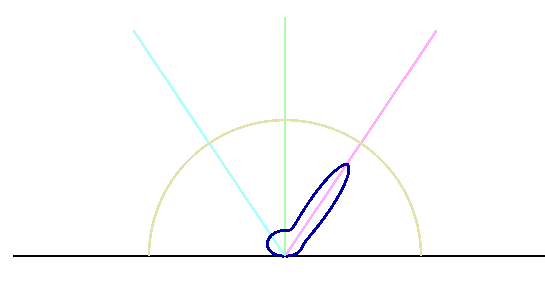
\includegraphics[width=\linewidth]{./Imagens/brdfs/ashikhmin-shirley-close-to-original-polar-plot.png}
    \legend{ \small (b) \textit{Polar plot}}
\endminipage\hfill
\end{figure}

\begin{figure}[H]
    \caption{\small{Objetos 3D renderizados pelo experimento Ashikhmin-Shirley.}}\label{fig-ashikhmin-shirley-close-to-original-eqlang}
\minipage{0.32\textwidth}
  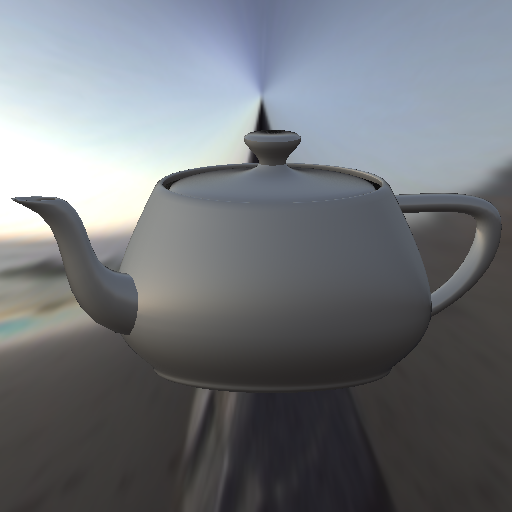
\includegraphics[width=\linewidth]{./Imagens/brdfs/ashikhmin-shirley-close-to-original-teapot.png}
    \legend{ \small (a) \textit{Teapot}}
\endminipage\hfill
\minipage{0.32\textwidth}
  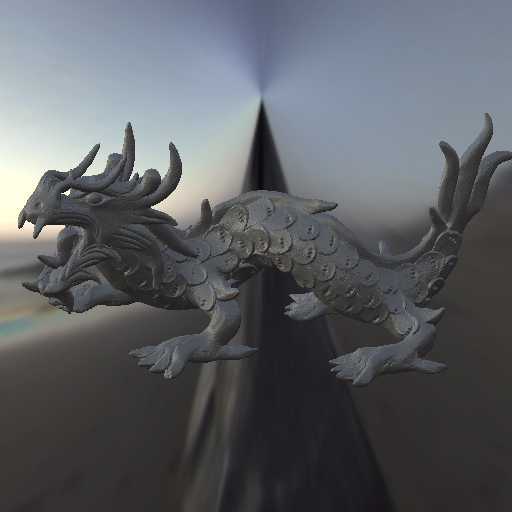
\includegraphics[width=\linewidth]{./Imagens/brdfs/ashikhmin-shirley-close-to-original-dragon.png}
    \legend{ \small (b) Dragão de Stanford}
\endminipage\hfill
\minipage{0.32\textwidth}%
  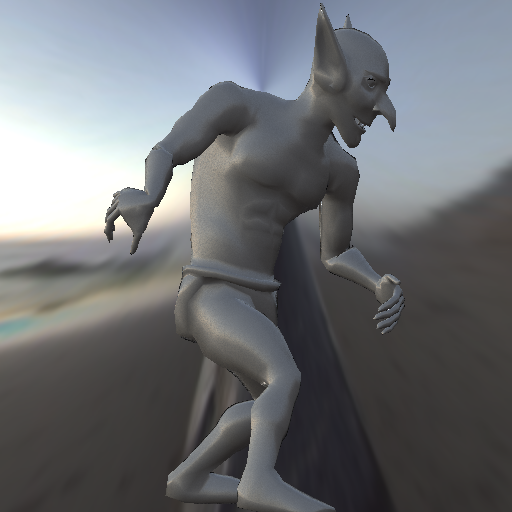
\includegraphics[width=\linewidth]{./Imagens/brdfs/ashikhmin-shirley-close-to-original-goblin.png}
    \legend{ \small (c) Goblin}
\endminipage
\end{figure}


\section{Experimento BRDF oren-nayar}

As equações que descrevem esse experimento se encontram em \autoref{fig-oren-nayar-eqlang-latex}. O código fonte de entrada para o compilador está dividido em duas partes, parte 1 está no \autoref{cod-oren-nayar-eqlang} e a segunda parte está em \autoref{cod-oren-nayar-eqlang-pt2}. A renderização dos objetos 3D usando essa BRDF se encontra em \autoref{fig-oren-nayar-eqlang}.

%%%%%%%%%%%%%%%%%%%%%%%%%%%%%%%%%%%%%%%%%%%%%%%%%
\subsection{Representação em documento \LaTeX{}}
%%%%%%%%%%%%%%%%%%%%%%%%%%%%%%%%%%%%%%%%%%%%%%%%%
\begin{figure}[H]
    \caption{\label{fig-oren-nayar-eqlang-latex} \small Equações da BRDF do experimento oren-nayar em documento \LaTeX{}.}
    \begin{center}
        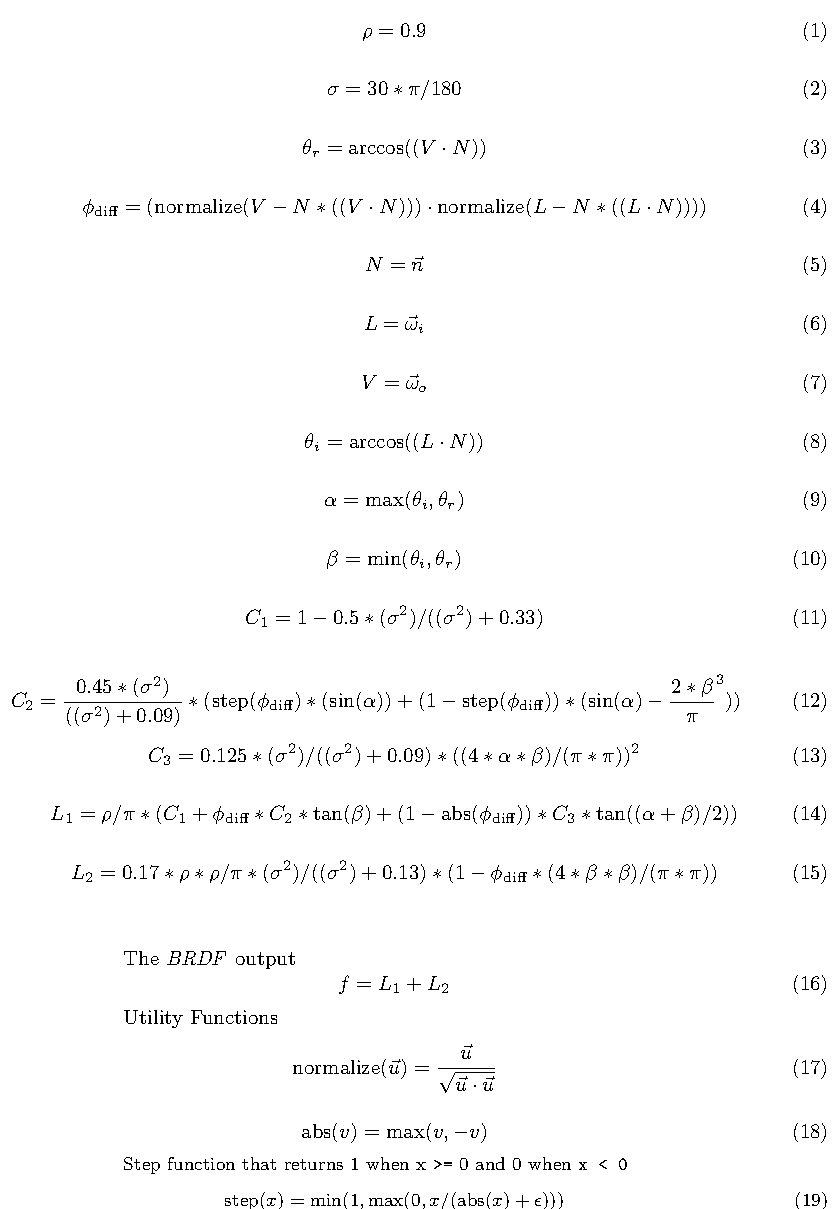
\includegraphics[scale=0.82]{./Imagens/brdfs/oren-nayar.pdf}
    \end{center}
\end{figure}

%%%%%%%%%%%%%%%%%%%%%%%%%%%%%%%%%%%%%%%%%%%%%%%%%
\subsection{Visualização do Resultado}
%%%%%%%%%%%%%%%%%%%%%%%%%%%%%%%%%%%%%%%%%%%%%%%%%
\begin{figure}[H]
    \caption{\small{Distribuição de Reflexão Especular e Difusa da BRDF}}\label{fig-oren-nayar-eqlang}
\minipage{0.48\textwidth}
    \vspace{42px}
  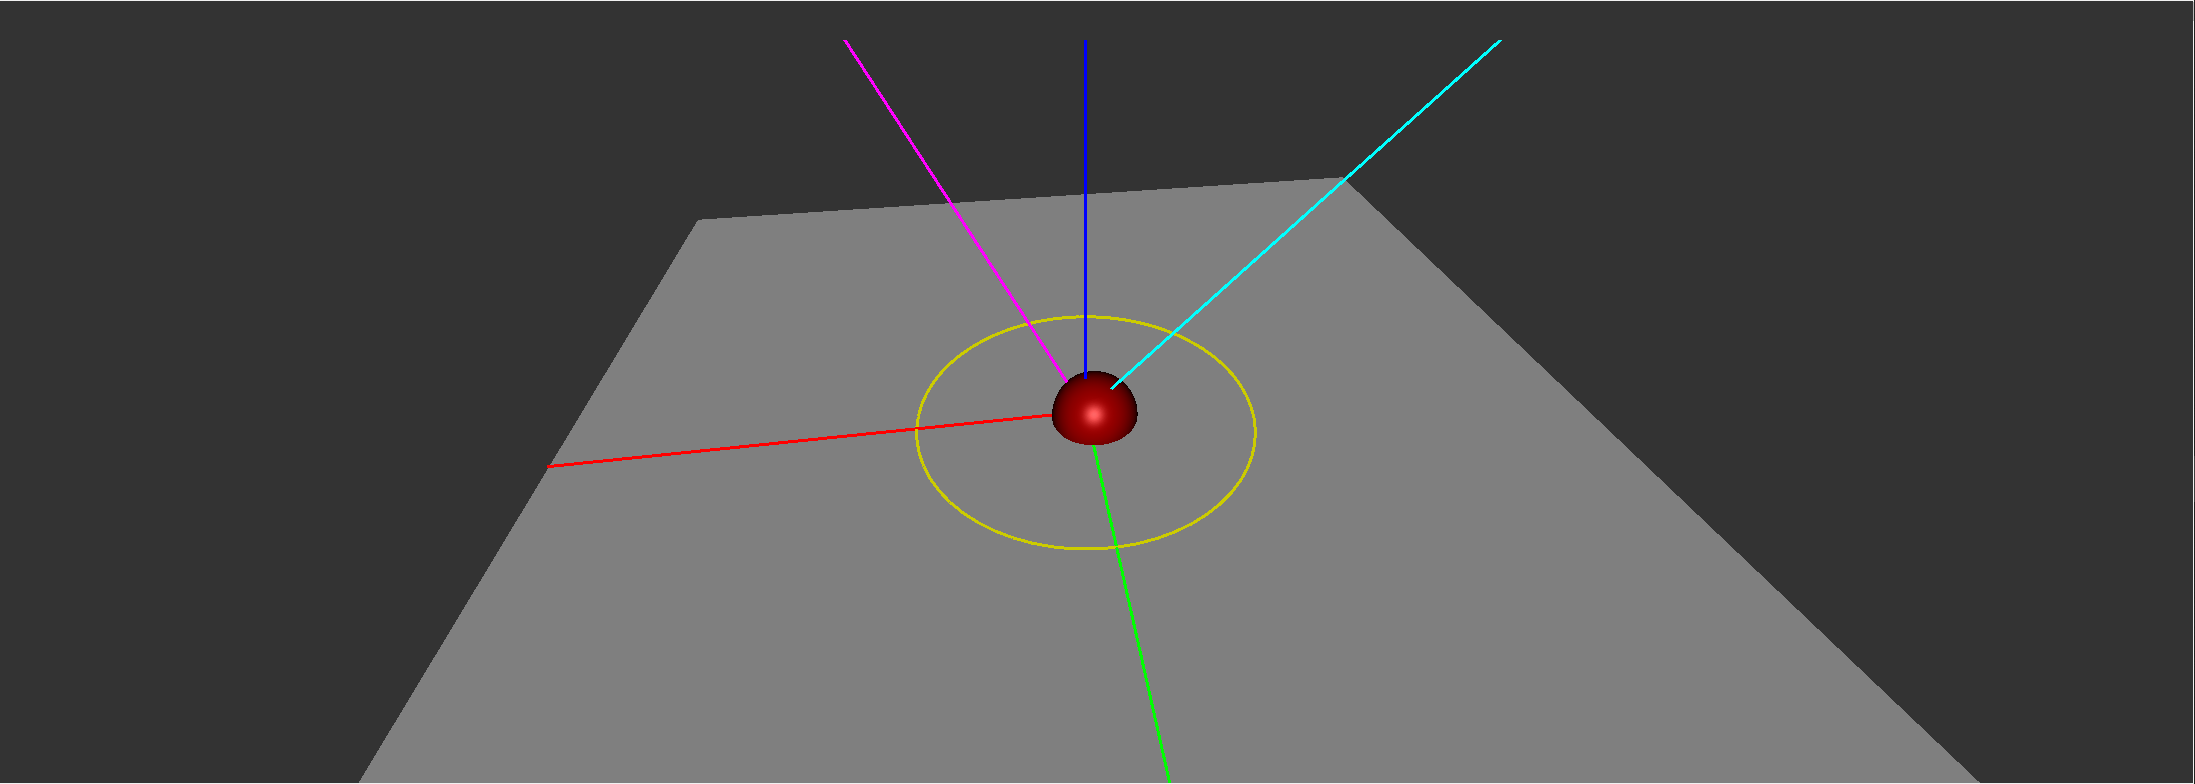
\includegraphics[width=\linewidth]{./Imagens/brdfs/oren-nayar-3D-plot}
    % \vspace{0.1px}
    \legend{ \small (a) 3D \textit{plot}}
\endminipage\hfill
\minipage{0.48\textwidth}
  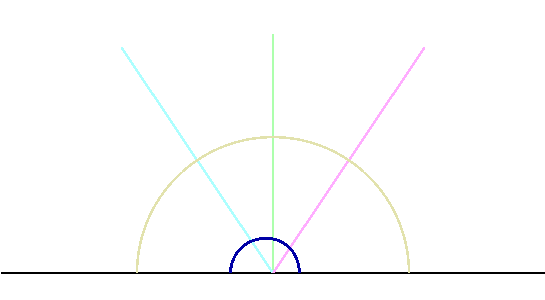
\includegraphics[width=\linewidth]{./Imagens/brdfs/oren-nayar-polar-plot.png}
    \legend{ \small (b) \textit{Polar plot}}
\endminipage\hfill
\end{figure}

\begin{figure}[H]
    \caption{\small{Objetos 3D renderizados por este experimento}}\label{fig-oren-nayar-eqlang}
\minipage{0.32\textwidth}
  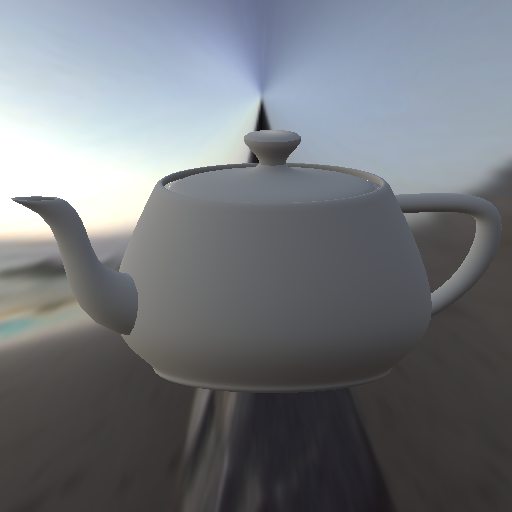
\includegraphics[width=\linewidth]{./Imagens/brdfs/oren-nayar-teapot.png}
    \legend{ \small (a) \textit{Teapot}}
\endminipage\hfill
\minipage{0.32\textwidth}
  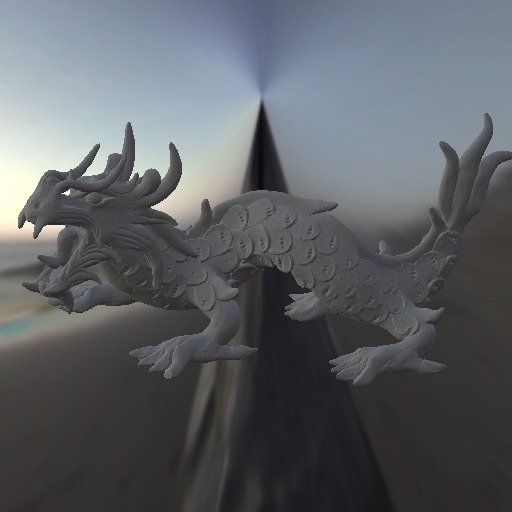
\includegraphics[width=\linewidth]{./Imagens/brdfs/oren-nayar-dragon.png}
    \legend{ \small (b) Dragão de Stanford}
\endminipage\hfill
\minipage{0.32\textwidth}%
  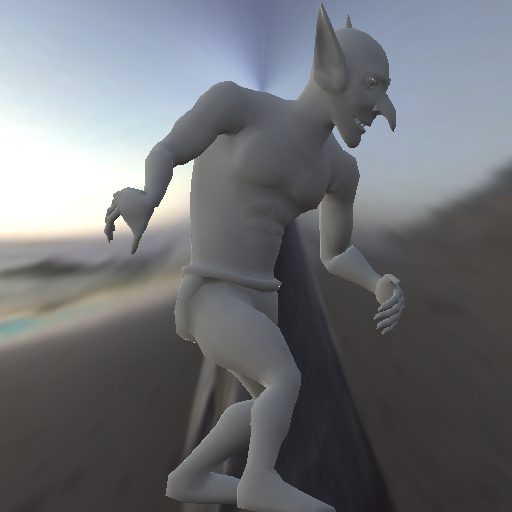
\includegraphics[width=\linewidth]{./Imagens/brdfs/oren-nayar-goblin.png}
    \legend{ \small (c) Goblin}
\endminipage
\end{figure}

%%%%%%%%%%%%%%%%%%%%%%%%%%%%%%%%%%%%%%%%%%%%%%%%%
\subsection{Código GLSL Gerado}
%%%%%%%%%%%%%%%%%%%%%%%%%%%%%%%%%%%%%%%%%%%%%%%%%
\begin{codigo}[H]
    \caption{\small Saida do compilador, código GLSL da BRDF deste experimento (parte 1). }
    \label{cod-oren-nayar-eqlang-declarations}
\begin{lstlisting}[language=C, inputencoding=utf8]
\end{lstlisting}
\end{codigo}

\begin{codigo}[H]
    \caption{\small Saida do compilador, código GLSL da BRDF deste experimento  (parte 2). }
    \label{cod-oren-nayar-eqlang}
\begin{lstlisting}[language=C, inputencoding=utf8]
\end{lstlisting}
\end{codigo}

%%%%%%%%%%%%%%%%%%%%%%%%%%%%%%%%%%%%%%%%%%%%%%%%%
\subsection{Código Fonte em \texttt{EquationLang}}
%%%%%%%%%%%%%%%%%%%%%%%%%%%%%%%%%%%%%%%%%%%%%%%%%
\begin{codigo}[H]
    \caption{\small Código fonte da BRDF deste experimento (parte 1).}
    \label{cod-oren-nayar-eqlang}
\begin{lstlisting}[language=tex, frame=none, inputencoding=utf8]
\end{lstlisting}
\end{codigo}

\section{Experimento BRDF Ashikhmin-Shirley Alternativa}


Nesse caso, foi realizado uma versão alternativa do experimento da \autoref{sec:ashikhmin-shirley}. As equações na \autoref{fig-ashikhmin-shirley-alternative-eqlang-latex} estão simplicadas e algumas equações foram comprimidas em uma só. Além disso, nessa versão, foram escolhidas diferentes constantes, como cor difusa, fatores de multiplicação, entre outros. Código fonte em \texttt{EquationLang} disponível no \autoref{cod-ashikhmin-shirley-alternative-eqlang}. Os códigos gerados em GLSL estão no \autoref{cod-ashikhmin-shirley-alternative-glsl-pt-1} e \autoref{cod-ashikhmin-shirley-alternative-glsl-pt-2}. Objetos 3D renderizados pode ser vistos na \autoref{fig-ashikhmin-shirley-alternative-eqlang} e os plots estão na \autoref{fig-ashikhmin-shirley-alternative-plots}.
%%%%%%%%%%%%%%%%%%%%%%%%%%%%%%%%%%%%%%%%%%%%%%%%%
\subsection{Representação em documento \LaTeX{}}
%%%%%%%%%%%%%%%%%%%%%%%%%%%%%%%%%%%%%%%%%%%%%%%%%
\begin{figure}[H]
    \caption{\label{fig-ashikhmin-shirley-alternative-eqlang-latex} \small Equações da BRDF do experimento ashikhmin-shirley-alternative em documento \LaTeX{}.}
    \begin{center}
        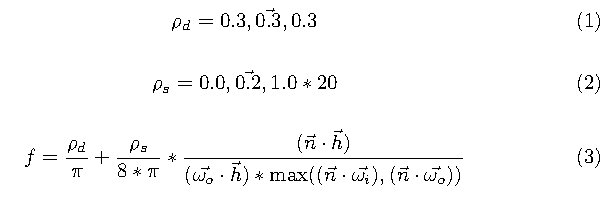
\includegraphics[scale=0.92]{./Imagens/brdfs/ashikhmin-shirley-alternative.pdf}
    \end{center}
\end{figure}

%%%%%%%%%%%%%%%%%%%%%%%%%%%%%%%%%%%%%%%%%%%%%%%%%
\subsection{Visualização do Resultado}
%%%%%%%%%%%%%%%%%%%%%%%%%%%%%%%%%%%%%%%%%%%%%%%%%
\begin{figure}[H]
    \caption{\small{Distribuição de Reflexão Especular e Difusa da BRDF}}\label{fig-ashikhmin-shirley-alternative-plots}
\minipage{0.48\textwidth}
    \vspace{42px}
  
\includegraphics[width=\linewidth]{./Imagens/brdfs/ashikhmin-shirley-alternative-3D-plot}
    % \vspace{0.1px}
    \legend{ \small (a) 3D \textit{plot}}
\endminipage\hfill
\minipage{0.48\textwidth}
  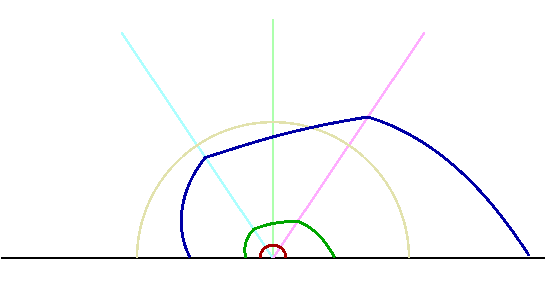
\includegraphics[width=\linewidth]{./Imagens/brdfs/ashikhmin-shirley-alternative-polar-plot.png}
    \legend{ \small (b) \textit{Polar plot}}
\endminipage\hfill
\end{figure}

\begin{figure}[H]
    \caption{\small{Objetos 3D renderizados por este experimento}}\label{fig-ashikhmin-shirley-alternative-eqlang}
\minipage{0.32\textwidth}
  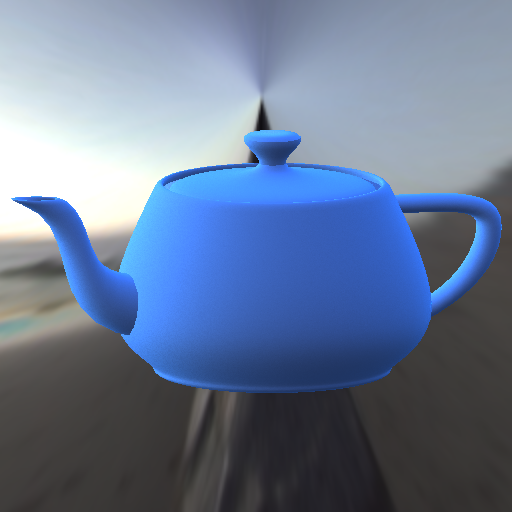
\includegraphics[width=\linewidth]{./Imagens/brdfs/ashikhmin-shirley-alternative-teapot.png}
    \legend{ \small (a) \textit{Teapot}}
\endminipage\hfill
\minipage{0.32\textwidth}
  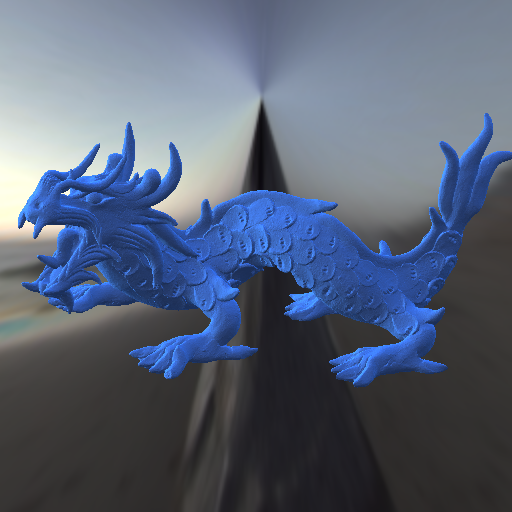
\includegraphics[width=\linewidth]{./Imagens/brdfs/ashikhmin-shirley-alternative-dragon.png}
    \legend{ \small (b) Dragão de Stanford}
\endminipage\hfill
\minipage{0.32\textwidth}%
  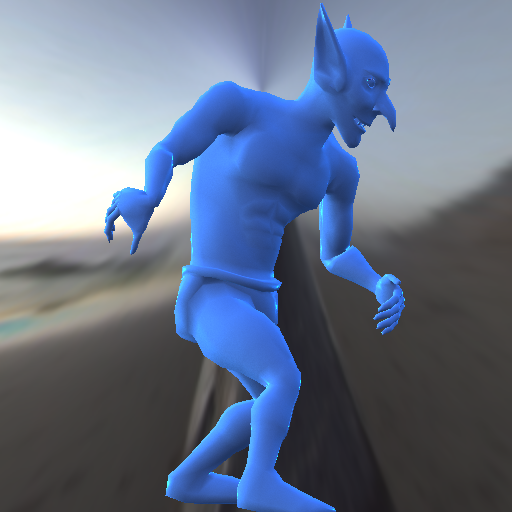
\includegraphics[width=\linewidth]{./Imagens/brdfs/ashikhmin-shirley-alternative-goblin.png}
    \legend{ \small (c) Goblin}
\endminipage
\end{figure}

%%%%%%%%%%%%%%%%%%%%%%%%%%%%%%%%%%%%%%%%%%%%%%%%%
\subsection{Código GLSL Gerado}
%%%%%%%%%%%%%%%%%%%%%%%%%%%%%%%%%%%%%%%%%%%%%%%%%
\begin{codigo}[H]
    \caption{\small Saida do compilador, código GLSL da BRDF deste experimento (parte 1). }
    \label{cod-ashikhmin-shirley-alternative-glsl-pt-1}
\begin{lstlisting}[language=C, inputencoding=utf8]
analytic ::begin parameters
#[type][name][min val][max val][default val]
::end parameters
::begin shader
//////////// START OF BUILTINS DECLARTION ////////////
vec3 var_0_vec_h;
vec3 var_3_vec_n;
float var_10_theta_h;
float var_11_theta_d;
float var_1_pi;
float var_2_epsilon;
vec3 var_4_vec_omega_i;
float var_5_theta_i;
float var_6_phi_i;
vec3 var_7_vec_omega_o;
float var_8_theta_o;
float var_9_phi_o;
//////////// END OF BUILTINS DECLARTION ////////////

//////////// START OF USER DECLARED ////////////
vec3 var_12_rho_d;
vec3 var_13_rho_s;
vec3 var_14_f;
//////////// END OF USER DECLARED ////////////
\end{lstlisting}
\end{codigo}

\begin{codigo}[H]
    \caption{\small Saida do compilador, código GLSL da BRDF deste experimento  (parte 2). }
    \label{cod-ashikhmin-shirley-alternative-glsl-pt-2}
\begin{lstlisting}[language=C, inputencoding=utf8]
//////////// START FUNCTIONS DECLARATIONS ////////////
//////////// END FUNCTIONS DECLARATIONS ////////////

vec3 BRDF(vec3 L, vec3 V, vec3 N, vec3 X, vec3 Y) {

  //////////// START OF BUILTINS INITIALIZATION ////////////
  var_0_vec_h = normalize(L + V);
  var_3_vec_n = normalize(N);
  var_1_pi = 3.141592653589793;
  var_2_epsilon = 1.192092896e-07;
  var_4_vec_omega_i = L;
  var_5_theta_i = atan(var_4_vec_omega_i.y, var_4_vec_omega_i.x);
  var_6_phi_i = atan(sqrt(var_4_vec_omega_i.y * var_4_vec_omega_i.y +
                          var_4_vec_omega_i.x * var_4_vec_omega_i.x),
                     var_4_vec_omega_i.z);
  var_7_vec_omega_o = V;
  var_8_theta_o = atan(var_7_vec_omega_o.y, var_7_vec_omega_o.x);
  var_9_phi_o = atan(sqrt(var_7_vec_omega_o.y * var_7_vec_omega_o.y +
                          var_7_vec_omega_o.x * var_7_vec_omega_o.x),
                     var_7_vec_omega_o.z);
  var_10_theta_h = acos(dot(var_0_vec_h, N));
  var_11_theta_d = acos(dot(var_0_vec_h, var_4_vec_omega_i));
  //////////// END OF BUILTINS INITIALIZATION ////////////

  var_12_rho_d = vec3(0.3, 0.3, 0.3);
  var_13_rho_s = (vec3(0.0, 0.2, 1.0) * 20.0);
  var_14_f = ((var_12_rho_d / var_1_pi) +
              ((var_13_rho_s / (8.0 * var_1_pi)) *
               ((dot(var_3_vec_n, var_0_vec_h)) /
                ((dot(var_7_vec_omega_o, var_0_vec_h)) *
                 max((dot(var_3_vec_n, var_4_vec_omega_i)),
                     (dot(var_3_vec_n, var_7_vec_omega_o)))))));

  return vec3(var_14_f);
}
\end{lstlisting}
\end{codigo}

%%%%%%%%%%%%%%%%%%%%%%%%%%%%%%%%%%%%%%%%%%%%%%%%%
\subsection{Código Fonte em \texttt{EquationLang}}
%%%%%%%%%%%%%%%%%%%%%%%%%%%%%%%%%%%%%%%%%%%%%%%%%
\begin{codigo}[H]
    \caption{\small Código fonte da BRDF deste experimento.}
    \label{cod-ashikhmin-shirley-alternative-eqlang}
\begin{lstlisting}[language=tex, frame=none, inputencoding=utf8]

\begin{document}

\begin{equation}
    \rho_{d} = \vec{0.3,0.3,0.3}
\end{equation}

\begin{equation}
    \rho_{s} = \vec{0.0,0.2,1.0}*20
\end{equation}

\begin{equation}
f = \frac{\rho_{d}}{\pi} + \frac{\rho_{s}}{8*\pi} *
\frac{({\vec{n}}\cdot{\vec{h}})}
{({\vec{\omega_{o}}}\cdot{\vec{h}}) *
\max(({\vec{n}}\cdot{\vec{\omega_{i}}}),
({\vec{n}}\cdot{\vec{\omega_{o}}}))}
\end{equation}

\end{lstlisting}
\end{codigo}


\section{Experimento BRDF Cook-Torrance Alternativa}
\label{section-experiment-cook-torrance-alternative}

Este experimento é uma versão alternativa da realizada na \autoref{sec:cook-torrance}. As equações apresentadas na \autoref{fig-cook-torrance-alternative-eqlang-latex} incorporam a equação do efeito Fresnel e utilizam constantes distintas. O código-fonte em \texttt{EquationLang} pode ser consultado no \autoref{cod-cook-torrance-alternative-eqlang}. O código gerado em GLSL está no \autoref{cod-cook-torrance-alternative-glsl-pt-1} e no \autoref{cod-cook-torrance-alternative-glsl-pt-2}. Objetos 3D renderizados podem ser vistos na \autoref{fig-cook-torrance-alternative-eqlang} e os \textit{plots} estão na \autoref{fig-cook-torrance-alternative-plots}.


%%%%%%%%%%%%%%%%%%%%%%%%%%%%%%%%%%%%%%%%%%%%%%%%%
\subsection{Representação em documento \LaTeX{}}
%%%%%%%%%%%%%%%%%%%%%%%%%%%%%%%%%%%%%%%%%%%%%%%%%
\begin{figure}[H]
    \caption{\label{fig-cook-torrance-alternative-eqlang-latex}
    \small Equações da BRDF do experimento Cook-Torrance$_2$ (alternativa) em documento \LaTeX{}.}
    \begin{center}
        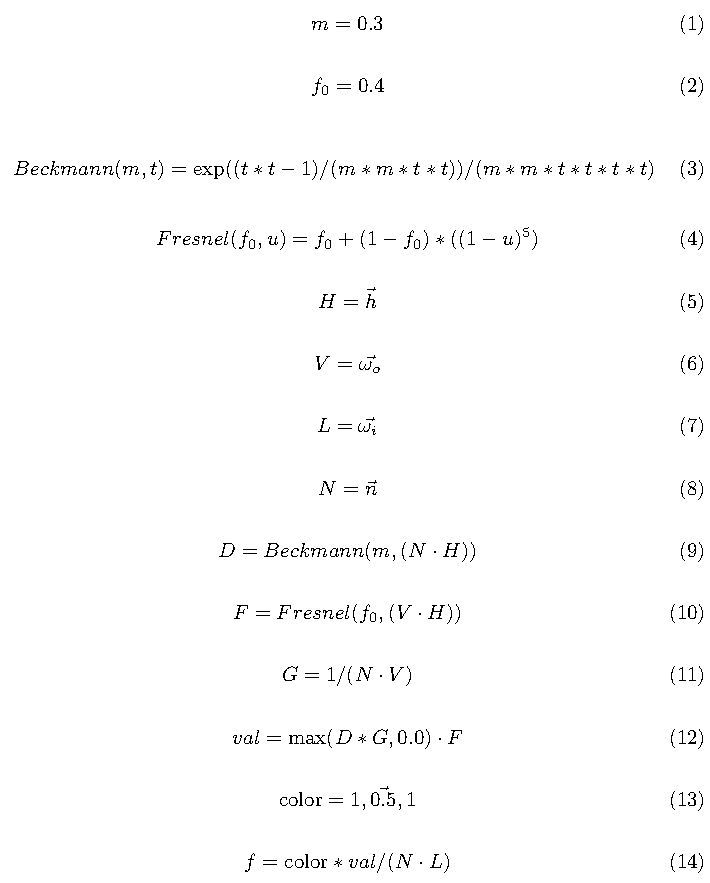
\includegraphics[scale=0.92]{./Imagens/brdfs/cook-torrance-alternative.pdf}
    \end{center}
\end{figure}

%%%%%%%%%%%%%%%%%%%%%%%%%%%%%%%%%%%%%%%%%%%%%%%%%
\subsection{Código Fonte em \texttt{EquationLang}}
%%%%%%%%%%%%%%%%%%%%%%%%%%%%%%%%%%%%%%%%%%%%%%%%%
\begin{codigo}[H]
    \caption{\small Código fonte da BRDF do experimento Cook-Torrance$_2$.}
    \label{cod-cook-torrance-alternative-eqlang}
\begin{lstlisting}[language=tex, frame=none, inputencoding=utf8]
\begin{equation}
    m = 0.3
\end{equation}
\begin{equation}
    f_0 = 0.4
\end{equation}
\begin{equation}
Beckmann(m, t) = \exp((t*t-1)/(m*m*t*t)) / (m*m*t*t*t*t)
\end{equation}
\begin{equation}
    Fresnel(f_0, u) = f_0 + (1 - f_0) * ((1-u)^ 5)
\end{equation}
\begin{equation}
    H = \vec{h}
\end{equation}
\begin{equation}
    V = \vec{\omega_o}
\end{equation}
\begin{equation}
    L = \vec{\omega_{i}}
\end{equation}
\begin{equation}
    N = \vec{n}
\end{equation}
\begin{equation}
    D = Beckmann(m,  (N \cdot H) )
\end{equation}
\begin{equation}
    F = Fresnel(f_0,  (V \cdot H) )
\end{equation}
\begin{equation}
G = 1/(N \cdot V)
\end{equation}
\begin{equation}
    val = \max(D * G, 0.0) \cdot F
\end{equation}
\begin{equation}
    \text{color} = \vec{1,0.5,1}
\end{equation}
\begin{equation}
    f = \text{color} * val / (N \cdot L)
\end{equation}
\end{lstlisting}
\end{codigo}

%%%%%%%%%%%%%%%%%%%%%%%%%%%%%%%%%%%%%%%%%%%%%%%%%
\subsection{Código GLSL Gerado}
%%%%%%%%%%%%%%%%%%%%%%%%%%%%%%%%%%%%%%%%%%%%%%%%%
\begin{codigo}[H]
    \caption{\small Saída do compilador: código GLSL da BRDF do experimento Cook-Torrance$_2$ (parte 1 de 2).}
    \label{cod-cook-torrance-alternative-glsl-pt-1}
\begin{lstlisting}[language=C, inputencoding=utf8]
analytic ::begin parameters
#[type][name][min val][max val][default val]
::end parameters
::begin shader
//////////// START OF BUILTINS DECLARTION ////////////
vec3 var_0_vec_h;
vec3 var_3_vec_n;
float var_10_theta_h;
float var_11_theta_d;
float var_1_pi;
float var_2_epsilon;
vec3 var_4_vec_omega_i;
float var_5_theta_i;
float var_6_phi_i;
vec3 var_7_vec_omega_o;
float var_8_theta_o;
float var_9_phi_o;
//////////// END OF BUILTINS DECLARTION ////////////
//////////// START OF USER DECLARED ////////////
vec3 var_12_V;
vec3 var_13_L;
float var_17_f_0;
float var_15_m;
vec3 var_20_H;
vec3 var_21_text_color;
vec3 var_22_N;
float var_23_D;
float var_24_G;
float var_25_F;
float var_26_val;
vec3 var_27_f;
\end{lstlisting}
\end{codigo}

\begin{codigo}[H]
    \caption{\small Saída do compilador: código GLSL da BRDF do experimento Cook-Torrance$_2$ (parte 2 de 2).}
    \label{cod-cook-torrance-alternative-glsl-pt-2}
\begin{lstlisting}[language=C, inputencoding=utf8]
//////////// END OF USER DECLARED ////////////
//////////// START FUNCTIONS DECLARATIONS ////////////
float var_14_Beckmann(float var_15_m, float var_16_t) {
  return (exp((((((var_16_t * var_16_t) - 1.0)) /
                ((((var_15_m * var_15_m) * var_16_t) * var_16_t))))) /
          ((((((var_15_m * var_15_m) * var_16_t) * var_16_t) * var_16_t) *
            var_16_t)));
}
float var_18_Fresnel(float var_17_f_0, float var_19_u) {
  return (var_17_f_0 + (((1.0 - var_17_f_0)) * (pow(((1.0 - var_19_u)), 5.0))));
}
//////////// END FUNCTIONS DECLARATIONS ////////////
//////////// END FUNCTIONS DECLARATIONS ////////////
vec3 BRDF(vec3 L, vec3 V, vec3 N, vec3 X, vec3 Y) {
  //////////// START OF BUILTINS INITIALIZATION ////////////
  var_0_vec_h = normalize(L + V);
  var_3_vec_n = normalize(N);
  var_1_pi = 3.141592653589793;
  var_2_epsilon = 1.192092896e-07;
  var_4_vec_omega_i = L;
  var_5_theta_i = atan(var_4_vec_omega_i.y, var_4_vec_omega_i.x);
  var_6_phi_i = atan(sqrt(var_4_vec_omega_i.y * var_4_vec_omega_i.y +
                          var_4_vec_omega_i.x * var_4_vec_omega_i.x),
                     var_4_vec_omega_i.z);
  var_7_vec_omega_o = V;
  var_8_theta_o = atan(var_7_vec_omega_o.y, var_7_vec_omega_o.x);
  var_9_phi_o = atan(sqrt(var_7_vec_omega_o.y * var_7_vec_omega_o.y +
                          var_7_vec_omega_o.x * var_7_vec_omega_o.x),
                     var_7_vec_omega_o.z);
  var_10_theta_h = acos(dot(var_0_vec_h, N));
  var_11_theta_d = acos(dot(var_0_vec_h, var_4_vec_omega_i));
  //////////// END OF BUILTINS INITIALIZATION ////////////

  var_12_V = var_7_vec_omega_o;
  var_13_L = var_4_vec_omega_i;
  var_17_f_0 = 0.4;
  var_15_m = 0.3;
  var_20_H = var_0_vec_h;
  var_21_text_color = vec3(1.0, 0.5, 1.0);
  var_22_N = var_3_vec_n;
  var_23_D = var_14_Beckmann(var_15_m, (dot(var_22_N, var_20_H)));
  var_24_G = (1.0 / (dot(var_22_N, var_12_V)));
  var_25_F = var_18_Fresnel(var_17_f_0, (dot(var_12_V, var_20_H)));
  var_26_val = (max((var_23_D * var_24_G), 0.0) * var_25_F);
  var_27_f = ((var_21_text_color * var_26_val) / (dot(var_22_N, var_13_L)));

  return vec3(var_27_f);
}
\end{lstlisting}
\end{codigo}

%%%%%%%%%%%%%%%%%%%%%%%%%%%%%%%%%%%%%%%%%%%%%%%%%
\subsection{Visualização do Resultado}
%%%%%%%%%%%%%%%%%%%%%%%%%%%%%%%%%%%%%%%%%%%%%%%%%
\begin{figure}[H]
    \caption{\small{\textit{Plots} da distribuição de reflexão especular e difusa do experimento Cook-Torrance$_2$.}}
    \label{fig-cook-torrance-alternative-plots}
\minipage{0.48\textwidth}
    \vspace{42px}
  
\includegraphics[width=\linewidth]{./Imagens/brdfs/cook-torrance-alternative-3D-plot}
    % \vspace{0.1px}
    \legend{ \small (a) 3D \textit{plot}}
\endminipage\hfill
\minipage{0.48\textwidth}
  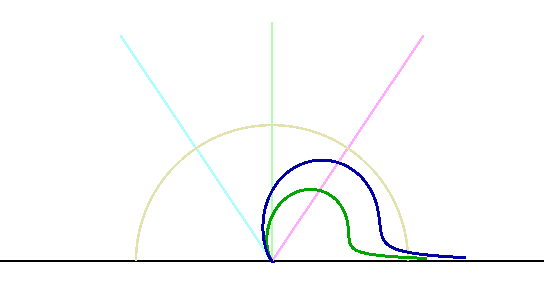
\includegraphics[width=\linewidth]{./Imagens/brdfs/cook-torrance-alternative-polar-plot-log.png}
    \legend{ \small (b) \textit{Polar plot}}
\endminipage\hfill
\end{figure}

\begin{figure}[H]
    \caption{\small{Objetos 3D renderizados pelo experimento Cook-Torrance$_2$.}}\label{fig-cook-torrance-alternative-eqlang}
\minipage{0.32\textwidth}
  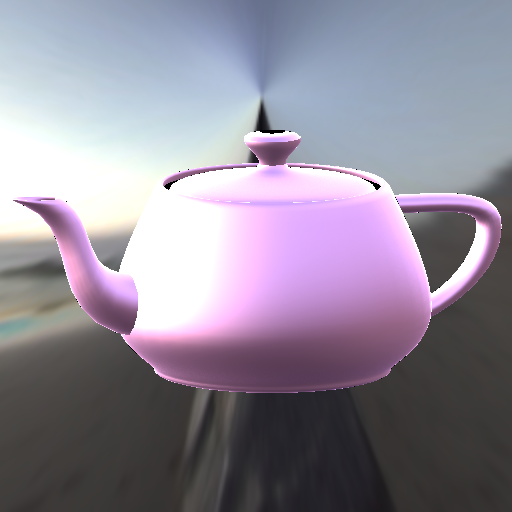
\includegraphics[width=\linewidth]{./Imagens/brdfs/cook-torrance-alternative-teapot.png}
    \legend{ \small (a) \textit{Teapot}}
\endminipage\hfill
\minipage{0.32\textwidth}
  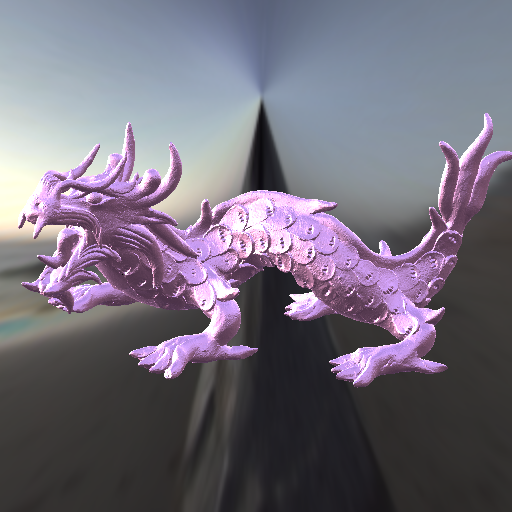
\includegraphics[width=\linewidth]{./Imagens/brdfs/cook-torrance-alternative-dragon.png}
    \legend{ \small (b) Dragão de Stanford}
\endminipage\hfill
\minipage{0.32\textwidth}%
  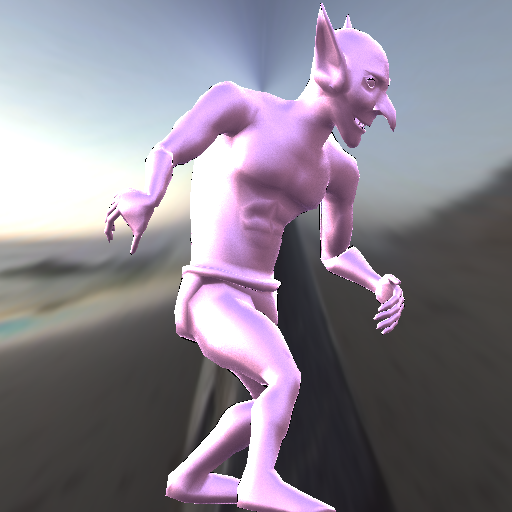
\includegraphics[width=\linewidth]{./Imagens/brdfs/cook-torrance-alternative-goblin.png}
    \legend{ \small (c) Goblin}
\endminipage
\end{figure}


\section{Experimento BRDF Dür}
\label{section-experiment-duer}

No artigo de Geisler-Moroder e Dür \cite{duer2010bounding}, são discutidas as limitações do modelo de reflexão de Ward, propondo uma abordagem para restringir o albedo e garantir a conservação de energia. Este experimento é baseado nessa BRDF com albedo restringido. As equações são apresentadas na \autoref{fig-duer-eqlang-latex}, com o código fonte em \texttt{EquationLang} disponível no \autoref{cod-duer-eqlang}. Os códigos gerados em GLSL podem ser vistos no \autoref{cod-duer-glsl-pt-1} e no \autoref{cod-duer-glsl-pt-2}. A renderização dos objetos 3D pode ser observada na \autoref{fig-duer-eqlang} e os \textit{plots} na \autoref{fig-duer-plots}.

%%%%%%%%%%%%%%%%%%%%%%%%%%%%%%%%%%%%%%%%%%%%%%%%%
\subsection{Representação em documento \LaTeX{}}
%%%%%%%%%%%%%%%%%%%%%%%%%%%%%%%%%%%%%%%%%%%%%%%%%
\begin{figure}[H]
    \caption{\label{fig-duer-eqlang-latex} \small Equações da BRDF do experimento Dür em documento \LaTeX{}.}
    \begin{center}
        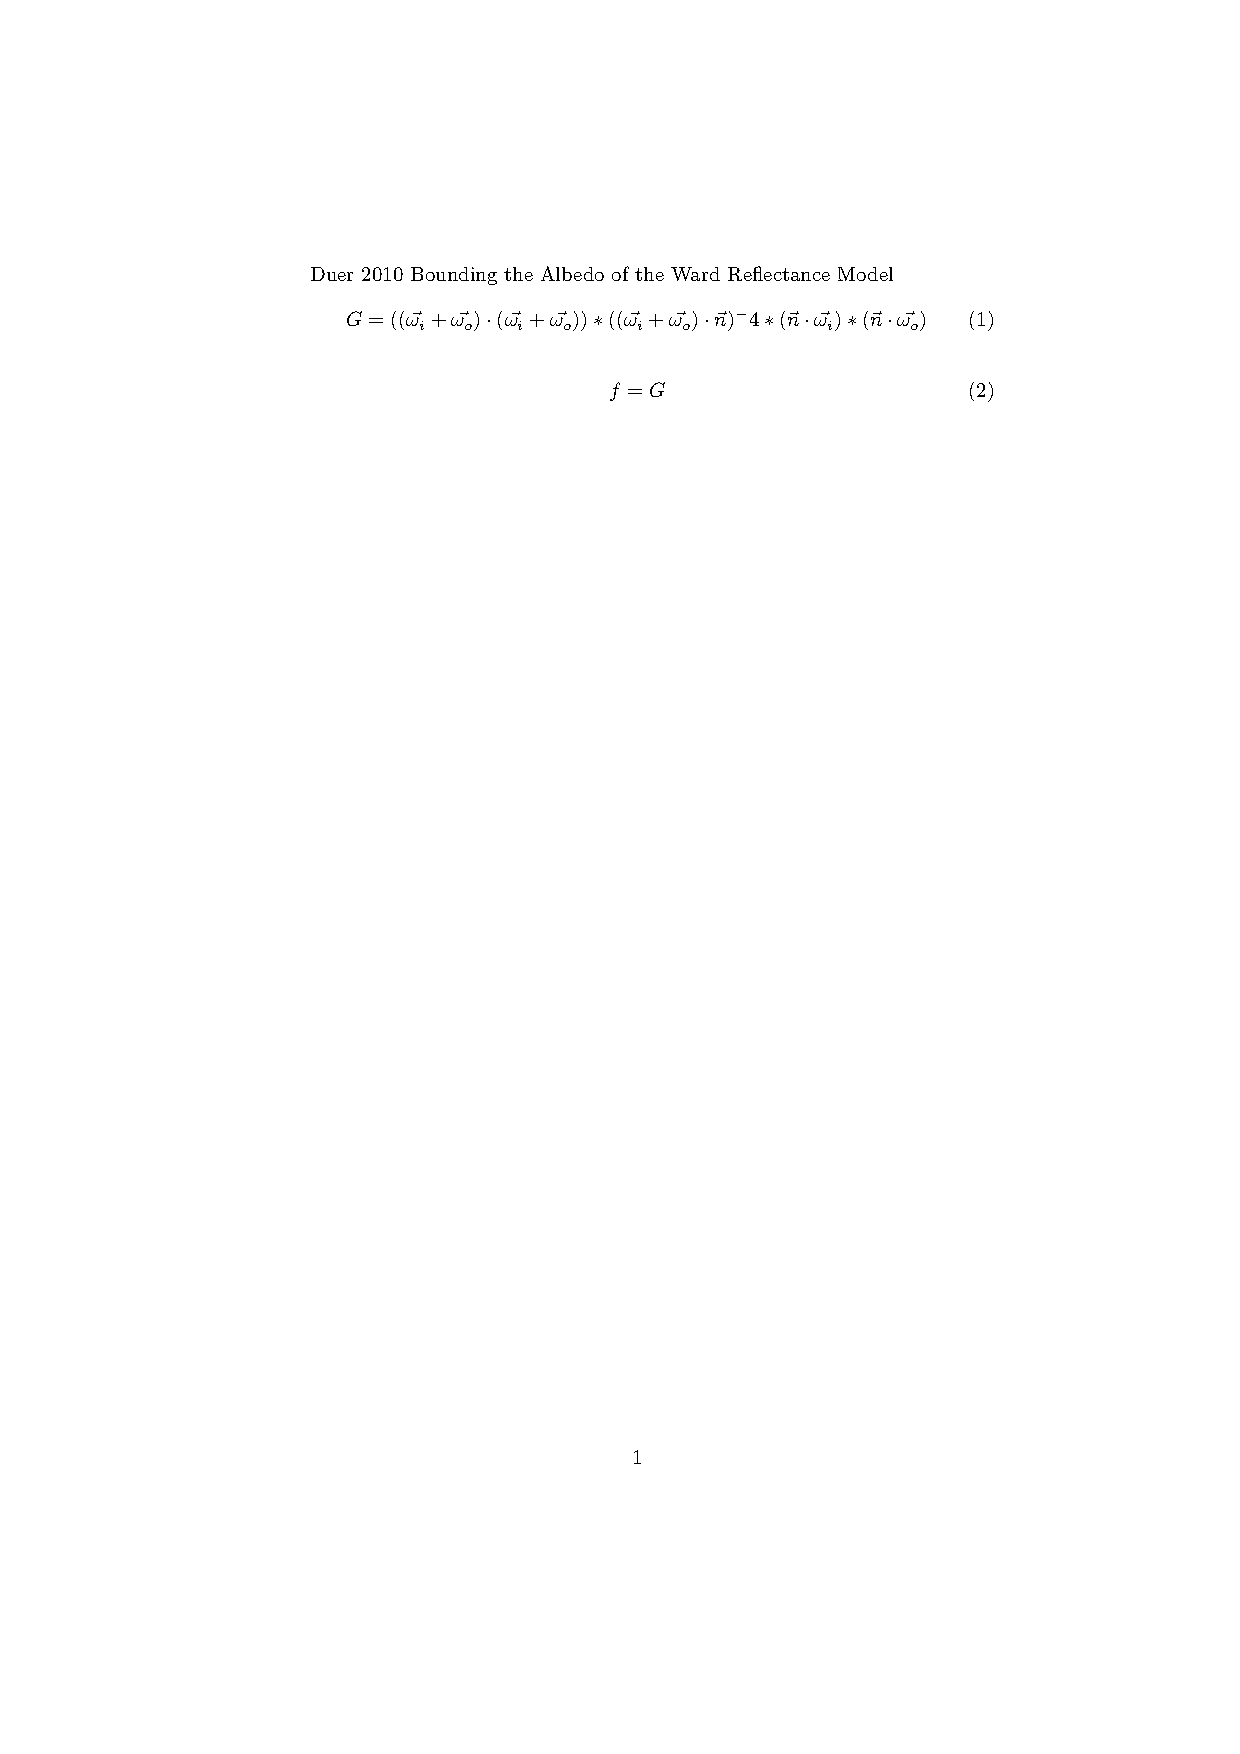
\includegraphics[scale=0.92]{./Imagens/brdfs/duer.pdf}
    \end{center}
\end{figure}

%%%%%%%%%%%%%%%%%%%%%%%%%%%%%%%%%%%%%%%%%%%%%%%%%
\subsection{Código Fonte em \texttt{EquationLang}}
%%%%%%%%%%%%%%%%%%%%%%%%%%%%%%%%%%%%%%%%%%%%%%%%%
\begin{codigo}[H]
    \caption{\small Código fonte da BRDF do experimento Dür.}
    \label{cod-duer-eqlang}
\begin{lstlisting}[language=tex, frame=none, inputencoding=utf8]
Duer 2010 Bounding the Albedo of the Ward Reflectance Model

\begin{equation}
G = ((\vec{\omega_i}+\vec{\omega_o}) \cdot(\vec{\omega_i}+\vec{\omega_o})) * ((\vec{\omega_i}+\vec{\omega_o}) \cdot \vec{n})^-4
    * (\vec{n} \cdot \vec{\omega_i})*(\vec{n} \cdot \vec{\omega_o})
\end{equation}

\begin{equation}
f =  G
\end{equation}
\end{lstlisting}
\end{codigo}

%%%%%%%%%%%%%%%%%%%%%%%%%%%%%%%%%%%%%%%%%%%%%%%%%
\subsection{Código GLSL Gerado}
%%%%%%%%%%%%%%%%%%%%%%%%%%%%%%%%%%%%%%%%%%%%%%%%%
\begin{codigo}[H]
    \caption{\small Saída do compilador: código GLSL da BRDF do experimento Dür (parte 1 de 2).}
    \label{cod-duer-glsl-pt-1}
\begin{lstlisting}[language=C, inputencoding=utf8]
analytic ::begin parameters
#[type][name][min val][max val][default val]
::end parameters
::begin shader
//////////// START OF BUILTINS DECLARTION ////////////
vec3 var_0_vec_h;
vec3 var_3_vec_n;
float var_10_theta_h;
float var_11_theta_d;
float var_1_pi;
float var_2_epsilon;
vec3 var_4_vec_omega_i;
float var_5_theta_i;
float var_6_phi_i;
vec3 var_7_vec_omega_o;
float var_8_theta_o;
float var_9_phi_o;
//////////// END OF BUILTINS DECLARTION ////////////
//////////// START OF USER DECLARED ////////////
float var_12_G;
float var_13_f;
//////////// END OF USER DECLARED ////////////
//////////// START FUNCTIONS DECLARATIONS ////////////
//////////// END FUNCTIONS DECLARATIONS ////////////

\end{lstlisting}
\end{codigo}

\begin{codigo}[H]
    \caption{\small Saída do compilador: código GLSL da BRDF do experimento Dür (parte 2 de 2).}
    \label{cod-duer-glsl-pt-2}
\begin{lstlisting}[language=C, inputencoding=utf8]
vec3 BRDF(vec3 L, vec3 V, vec3 N, vec3 X, vec3 Y) {

  //////////// START OF BUILTINS INITIALIZATION ////////////
  var_0_vec_h = normalize(L + V);
  var_3_vec_n = normalize(N);
  var_1_pi = 3.141592653589793;
  var_2_epsilon = 1.192092896e-07;
  var_4_vec_omega_i = L;
  var_5_theta_i = atan(var_4_vec_omega_i.y, var_4_vec_omega_i.x);
  var_6_phi_i = atan(sqrt(var_4_vec_omega_i.y * var_4_vec_omega_i.y +
                          var_4_vec_omega_i.x * var_4_vec_omega_i.x),
                     var_4_vec_omega_i.z);
  var_7_vec_omega_o = V;
  var_8_theta_o = atan(var_7_vec_omega_o.y, var_7_vec_omega_o.x);
  var_9_phi_o = atan(sqrt(var_7_vec_omega_o.y * var_7_vec_omega_o.y +
                          var_7_vec_omega_o.x * var_7_vec_omega_o.x),
                     var_7_vec_omega_o.z);
  var_10_theta_h = acos(dot(var_0_vec_h, N));
  var_11_theta_d = acos(dot(var_0_vec_h, var_4_vec_omega_i));
  //////////// END OF BUILTINS INITIALIZATION ////////////

  var_12_G =
      ((((dot(((var_4_vec_omega_i + var_7_vec_omega_o)),
              ((var_4_vec_omega_i + var_7_vec_omega_o)))) *
         pow((dot(((var_4_vec_omega_i + var_7_vec_omega_o)), var_3_vec_n)),
             (-4.0))) *
        (dot(var_3_vec_n, var_4_vec_omega_i))) *
       (dot(var_3_vec_n, var_7_vec_omega_o)));
  var_13_f = var_12_G;

  return vec3(var_13_f);
}
\end{lstlisting}
\end{codigo}


%%%%%%%%%%%%%%%%%%%%%%%%%%%%%%%%%%%%%%%%%%%%%%%%%
\subsection{Visualização do Resultado}
%%%%%%%%%%%%%%%%%%%%%%%%%%%%%%%%%%%%%%%%%%%%%%%%%
\begin{figure}[H]
    \caption{\small{\textit{Plots} da distribuição de reflexão especular e difusa do experimento Dür.}}
    \label{fig-duer-plots}
\minipage{0.48\textwidth}
    \vspace{42px}
  
\includegraphics[width=\linewidth]{./Imagens/brdfs/duer-3D-plot}
    % \vspace{0.1px}
    \legend{ \small (a) 3D \textit{plot}}
\endminipage\hfill
\minipage{0.48\textwidth}
  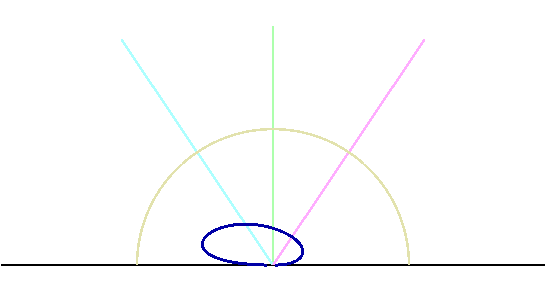
\includegraphics[width=\linewidth]{./Imagens/brdfs/duer-polar-plot.png}
    \legend{ \small (b) \textit{Polar plot}}
\endminipage\hfill
\end{figure}

\begin{figure}[H]
    \caption{\small{Objetos 3D renderizados pelo experimento Dür.}}
    \label{fig-duer-eqlang}
\minipage{0.32\textwidth}
  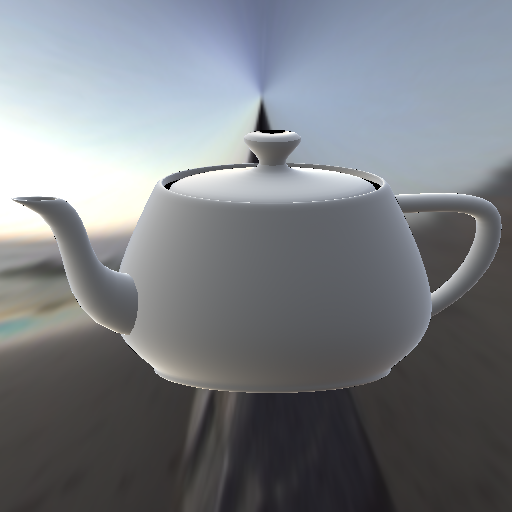
\includegraphics[width=\linewidth]{./Imagens/brdfs/duer-teapot.png}
    \legend{ \small (a) \textit{Teapot}}
\endminipage\hfill
\minipage{0.32\textwidth}
  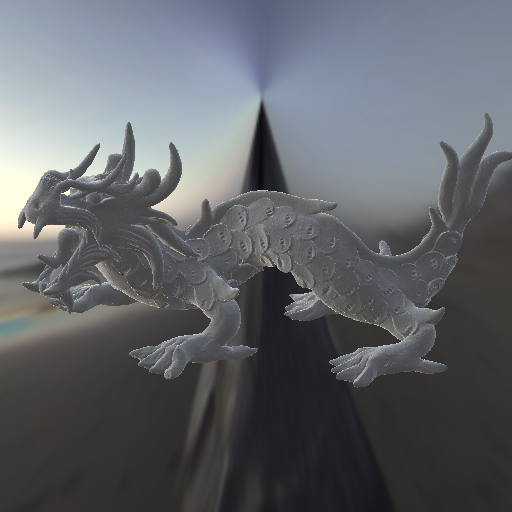
\includegraphics[width=\linewidth]{./Imagens/brdfs/duer-dragon.png}
    \legend{ \small (b) Dragão de Stanford}
\endminipage\hfill
\minipage{0.32\textwidth}%
  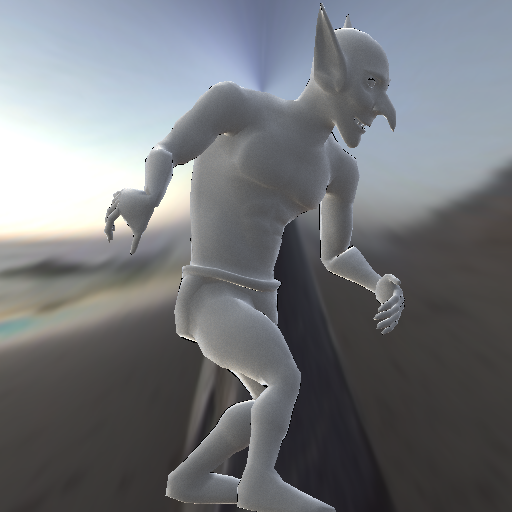
\includegraphics[width=\linewidth]{./Imagens/brdfs/duer-goblin.png}
    \legend{ \small (c) Goblin}
\endminipage
\end{figure}



\section{Experimento BRDF Edwards 2006}
\label{section-experiment-edwards-2006}

No artigo de Edwards et al. \cite{edwards2006halfway}, é apresentado o conceito do \textit{Halfway Vector Disk} como uma extensão para modelagem de BRDFs. Este método, usado neste experimento, propõe uma ideia geométrica que melhora a eficiência computacional. As equações principais são descritas na \autoref{fig-edwards-2006-eqlang-latex}, com o código fonte em \texttt{EquationLang} disponível no \autoref{cod-edwards-2006-eqlang}. Os códigos gerados em GLSL podem ser vistos no \autoref{cod-edwards-2006-glsl-pt-1} e no \autoref{cod-edwards-2006-glsl-pt-2}. A renderização de objetos 3D utilizando o método pode ser observada na \autoref{fig-edwards-2006-eqlang}, enquanto os \textit{plots} estão ilustrados na \autoref{fig-edwards-2006-plots}.

%%%%%%%%%%%%%%%%%%%%%%%%%%%%%%%%%%%%%%%%%%%%%%%%%
\subsection{Representação em documento \LaTeX{}}
%%%%%%%%%%%%%%%%%%%%%%%%%%%%%%%%%%%%%%%%%%%%%%%%%
\begin{figure}[H]
    \caption{\label{fig-edwards-2006-eqlang-latex} \small Equações da BRDF do experimento Edwards em documento \LaTeX{}.}
    \begin{center}
        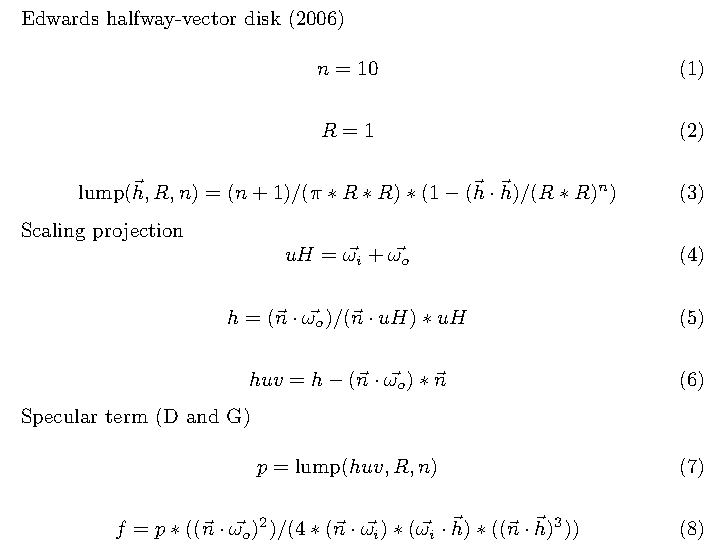
\includegraphics[scale=0.92]{./Imagens/brdfs/edwards-2006.pdf}
    \end{center}
\end{figure}

%%%%%%%%%%%%%%%%%%%%%%%%%%%%%%%%%%%%%%%%%%%%%%%%%
\subsection{Código GLSL Gerado}
%%%%%%%%%%%%%%%%%%%%%%%%%%%%%%%%%%%%%%%%%%%%%%%%%
\begin{codigo}[H]
    \caption{\small Saída do compilador: código GLSL da BRDF do experimento Edwards (parte 1 de 2).}
    \label{cod-edwards-2006-glsl-pt-1}
\begin{lstlisting}[language=C, inputencoding=utf8]
analytic ::begin parameters
#[type][name][min val][max val][default val]
::end parameters
::begin shader
//////////// START OF BUILTINS DECLARTION ////////////
vec3 var_0_vec_h;
vec3 var_3_vec_n;
float var_10_theta_h;
float var_11_theta_d;
float var_1_pi;
float var_2_epsilon;
vec3 var_4_vec_omega_i;
float var_5_theta_i;
float var_6_phi_i;
vec3 var_7_vec_omega_o;
float var_8_theta_o;
float var_9_phi_o;
//////////// END OF BUILTINS DECLARTION ////////////

//////////// START OF USER DECLARED ////////////
vec3 var_15_uH;
vec3 var_16_h;
float var_14_n;
vec3 var_17_huv;
float var_13_R;
float var_18_p;
float var_19_f;
\end{lstlisting}
\end{codigo}

\begin{codigo}[H]
    \caption{\small Saída do compilador: código GLSL da BRDF do experimento Edwards (parte 2 de 2).}
    \label{cod-edwards-2006-glsl-pt-2}
\begin{lstlisting}[language=C, inputencoding=utf8]
//////////// END OF USER DECLARED ////////////

//////////// START FUNCTIONS DECLARATIONS ////////////
float var_12_text_lump(vec3 var_0_vec_h, float var_13_R, float var_14_n) {
  return ((((var_14_n + 1.0)) / (((var_1_pi * var_13_R) * var_13_R))) *
          ((1.0 - ((dot(var_0_vec_h, var_0_vec_h)) /
                   pow(((var_13_R * var_13_R)), var_14_n)))));
}
//////////// END FUNCTIONS DECLARATIONS ////////////
vec3 BRDF(vec3 L, vec3 V, vec3 N, vec3 X, vec3 Y) {

  //////////// START OF BUILTINS INITIALIZATION ////////////
  var_0_vec_h = normalize(L + V);
  var_3_vec_n = normalize(N);
  var_1_pi = 3.141592653589793;
  var_2_epsilon = 1.192092896e-07;
  var_4_vec_omega_i = L;
  var_5_theta_i = atan(var_4_vec_omega_i.y, var_4_vec_omega_i.x);
  var_6_phi_i = atan(sqrt(var_4_vec_omega_i.y * var_4_vec_omega_i.y +
                          var_4_vec_omega_i.x * var_4_vec_omega_i.x),
                     var_4_vec_omega_i.z);
  var_7_vec_omega_o = V;
  var_8_theta_o = atan(var_7_vec_omega_o.y, var_7_vec_omega_o.x);
  var_9_phi_o = atan(sqrt(var_7_vec_omega_o.y * var_7_vec_omega_o.y +
                          var_7_vec_omega_o.x * var_7_vec_omega_o.x),
                     var_7_vec_omega_o.z);
  var_10_theta_h = acos(dot(var_0_vec_h, N));
  var_11_theta_d = acos(dot(var_0_vec_h, var_4_vec_omega_i));
  //////////// END OF BUILTINS INITIALIZATION ////////////

  var_15_uH = (var_4_vec_omega_i + var_7_vec_omega_o);
  var_16_h =
      (((dot(var_3_vec_n, var_7_vec_omega_o)) / (dot(var_3_vec_n, var_15_uH))) *
       var_15_uH);
  var_14_n = 10.0;
  var_17_huv =
      (var_16_h - ((dot(var_3_vec_n, var_7_vec_omega_o)) * var_3_vec_n));
  var_13_R = 1.0;
  var_18_p = var_12_text_lump(var_17_huv, var_13_R, var_14_n);
  var_19_f = ((var_18_p * (pow((dot(var_3_vec_n, var_7_vec_omega_o)), 2.0))) /
              ((((4.0 * (dot(var_3_vec_n, var_4_vec_omega_i))) *
                 (dot(var_4_vec_omega_i, var_0_vec_h))) *
                (pow((dot(var_3_vec_n, var_0_vec_h)), 3.0)))));

  return vec3(var_19_f);
}
\end{lstlisting}
\end{codigo}

%%%%%%%%%%%%%%%%%%%%%%%%%%%%%%%%%%%%%%%%%%%%%%%%%
\subsection{Código Fonte em \texttt{EquationLang}}
%%%%%%%%%%%%%%%%%%%%%%%%%%%%%%%%%%%%%%%%%%%%%%%%%
\begin{codigo}[H]
    \caption{\small Código fonte da BRDF do experimento Edwards.}
    \label{cod-edwards-2006-eqlang}
\begin{lstlisting}[language=tex, frame=none, inputencoding=utf8]
\begin{equation}
n = 10
\end{equation}

\begin{equation}
R = 1
\end{equation}

\begin{equation}
\text{lump}(\vec{h}, R, n) = (n+1)/(\pi*R*R) * (1-(\vec{h} \cdot \vec{h})/(R*R)^ n)
\end{equation}

Scaling projection
\begin{equation}
    uH = \vec{\omega_i}+\vec{\omega_o} % // unnormalized H
\end{equation}

\begin{equation}
    h = (\vec{n} \cdot \vec{\omega_o}) / (\vec{n} \cdot uH) * uH
\end{equation}

\begin{equation}
    huv = h - (\vec{n} \cdot \vec{\omega_o}) * \vec{n}
\end{equation}

Specular term (D and G)

\begin{equation}
    p = \text{lump}(huv, R, n)
\end{equation}

\begin{equation}
    f = p * ((\vec{n} \cdot \vec{\omega_o})^ 2)
        / (4 * (\vec{n} \cdot \vec{\omega_i}) * (\vec{\omega_i} \cdot \vec{h})
        * ((\vec{n} \cdot \vec{h})^ 3))
\end{equation}
\end{lstlisting}
\end{codigo}

%%%%%%%%%%%%%%%%%%%%%%%%%%%%%%%%%%%%%%%%%%%%%%%%%
\subsection{Visualização do Resultado}
%%%%%%%%%%%%%%%%%%%%%%%%%%%%%%%%%%%%%%%%%%%%%%%%%
\begin{figure}[H]
    \caption{\small{\textit{Plots} da distribuição de reflexão especular e difusa do experimento Edwards.}}
    \label{fig-edwards-2006-plots}
\minipage{0.48\textwidth}
    \vspace{42px}
  \includegraphics[width=\linewidth]{./Imagens/brdfs/edwards-2006-3D-plot}
    % \vspace{0.1px}
    \legend{ \small (a) 3D \textit{plot}}
\endminipage\hfill
\minipage{0.48\textwidth}
  \includegraphics[width=\linewidth]{./Imagens/brdfs/edwards-2006-polar-plot.png}
    \legend{ \small (b) \textit{Polar plot}}
\endminipage\hfill
\end{figure}

\begin{figure}[H]
    \caption{\small{Objetos 3D renderizados pelo experimento Edwards.}}\label{fig-edwards-2006-eqlang}
\minipage{0.32\textwidth}
  \includegraphics[width=\linewidth]{./Imagens/brdfs/edwards-2006-teapot.png}
    \legend{ \small (a) \textit{Teapot}}
\endminipage\hfill
\minipage{0.32\textwidth}
  \includegraphics[width=\linewidth]{./Imagens/brdfs/edwards-2006-dragon.png}
    \legend{ \small (b) Dragão de Stanford}
\endminipage\hfill
\minipage{0.32\textwidth}%
  \includegraphics[width=\linewidth]{./Imagens/brdfs/edwards-2006-goblin.png}
    \legend{ \small (c) Goblin}
\endminipage
\end{figure}


\section{Experimento BRDF Anisotrópica baseado em Kajiya-Kay (1989)}

A BRDF de especularidade anisotrópica, baseada no trabalho seminal de @@REF Kajiya-Kay de 1989, modela a reflexão especular em superfícies com características direcionais, como tecidos e cabelos. Esta abordagem captura de forma sofisticada a distribuição de luz em superfícies com orientação preferencial. As equações que descrevem esse experimento se encontram em \autoref{fig-kajiya-eqlang-latex}. O código fonte de entrada para o compilador está dividido em duas partes, parte 1 está no \autoref{cod-kajiya-eqlang} e a segunda parte está em \autoref{cod-kajiya-eqlang-pt2}. A redenrização de um objeto 3D usando essa BRDF esta em \autoref{fig-kajiya-eqlang}.

%%%%%%%%%%%%%%%%%%%%%%%%%%%%%%%%%%%%%%%%%%%%%%%%%
\subsection{Representação em documento \LaTeX{}}
%%%%%%%%%%%%%%%%%%%%%%%%%%%%%%%%%%%%%%%%%%%%%%%%%
\begin{figure}[H]
    \caption{\label{fig-kajiya-eqlang-latex} \small Equações da BRDF do experimento Kajiya-Kay em documento \LaTeX{}.}
    \begin{center}
        % \includegraphics[scale=1.1,width=\textwidth]{./Imagens/brdfs/aniso.pdf}
        \includegraphics[scale=0.92]{./Imagens/brdfs/aniso.pdf}
    \end{center}
\end{figure}

%%%%%%%%%%%%%%%%%%%%%%%%%%%%%%%%%%%%%%%%%%%%%%%%%
\subsection{Visualização do Resultado}
%%%%%%%%%%%%%%%%%%%%%%%%%%%%%%%%%%%%%%%%%%%%%%%%%

\begin{figure}[H]
    \caption{\small{Distribuição de Reflexão Especular e Difusa da BRDF Anisotrópica: Kajiya-Kay (1989)}}\label{fig-kajiya-eqlang}
\minipage{0.48\textwidth}
    \vspace{42px}
  \includegraphics[width=\linewidth]{./Imagens/brdfs/aniso-3D-plot}
    % \caption{\small{(a)}}\label{fig:awesome_image1}
    % \vspace{0.1px}
    \legend{ \small (a) 3D \textit{plot}}
\endminipage\hfill
\minipage{0.48\textwidth}
  \includegraphics[width=\linewidth]{./Imagens/brdfs/aniso-polar-plot.png}
    \legend{ \small (b) \textit{Polar plot}}
    % \caption{\small{(b)}}\label{fig:awesome_image1}
\endminipage\hfill
\end{figure}

\begin{figure}[H]
    % \caption{\small{Objetos 3D renderizado pelo código GLSL gerado o experimento BRDF Anisotrópica: Kajiya-Kay (1989)}}\label{fig-kajiya-eqlang}
    \caption{\small{Objetos 3D renderizado no experimento BRDF Anisotrópica: Kajiya-Kay (1989)}}\label{fig-kajiya-eqlang}
\minipage{0.32\textwidth}
  \includegraphics[width=\linewidth]{./Imagens/brdfs/aniso-teapot.png}
    % \caption{\small{(a)}}\label{fig:awesome_image1}
    \legend{ \small (a) \textit{Teapot}}
\endminipage\hfill
\minipage{0.32\textwidth}
  \includegraphics[width=\linewidth]{./Imagens/brdfs/aniso-dragon.png}
    \legend{ \small (b) Dragão de Stanford}
    % \caption{\small{(b)}}\label{fig:awesome_image1}
\endminipage\hfill
\minipage{0.32\textwidth}%
  \includegraphics[width=\linewidth]{./Imagens/brdfs/aniso-goblin.png}
    \legend{ \small (c) Goblin}
    % \caption{\small{(c)}}\label{fig:awesome_image1}
\endminipage
\end{figure}

%%%%%%%%%%%%%%%%%%%%%%%%%%%%%%%%%%%%%%%%%%%%%%%%%
\subsection{Código GLSL Gerado}
%%%%%%%%%%%%%%%%%%%%%%%%%%%%%%%%%%%%%%%%%%%%%%%%%
\begin{codigo}[H]
    \caption{\small Saida do compilador, código GLSL da BRDF do experimento baseado em Kajiya-Kay (parte 1). }
    \label{cod-kajiya-eqlang-declarations}
\begin{lstlisting}[language=C, inputencoding=utf8]
analytic
::begin parameters
# [type] [name] [min val] [max val] [default val]
::end parameters
::begin shader

//////////// START OF BUILTINS DECLARTION ////////////
vec3  var_0_vec_h;
vec3  var_3_vec_n;
float var_10_theta_h;
float var_11_theta_d;
float var_1_pi;
float var_2_epsilon;
vec3  var_4_vec_omega_i;
float var_5_theta_i;
float var_6_phi_i;
vec3  var_7_vec_omega_o;
float var_8_theta_o;
float var_9_phi_o;
//////////// END OF BUILTINS DECLARTION ////////////

//////////// START OF USER DECLARED ////////////
float var_12_text_roughness;
float var_13_text_glossiness;
vec3  var_16_X;
vec3  var_17_Y;
vec3  var_18_T;
vec3  var_19_L;
float var_20_text_sinAngleLT;
float var_21_text_spec;
float var_22_f;
//////////// END OF USER DECLARED ////////////
\end{lstlisting}
\end{codigo}

\begin{codigo}[H]
    \caption{\small Saida do compilador, código GLSL da BRDF do experimento baseado em Kajiya-Kay (parte 2). }
    \label{cod-kajiya-eqlang}
\begin{lstlisting}[language=C, inputencoding=utf8]
//////////// START FUNCTIONS DECLARATIONS ////////////
vec3 var_14_text_normalize(vec3 var_15_vec_u) {
    return (var_15_vec_u/sqrt(dot(var_15_vec_u,var_15_vec_u)));
}
//////////// END FUNCTIONS DECLARATIONS ////////////
vec3 BRDF(vec3 L, vec3 V, vec3 N, vec3 X, vec3 Y) {

//////////// START OF BUILTINS INITIALIZATION ////////////
  var_0_vec_h = normalize(L + V);
  var_3_vec_n = normalize(N);
  var_1_pi = 3.141592653589793;
  var_2_epsilon = 1.192092896e-07;
  var_4_vec_omega_i = L;
  var_5_theta_i = atan(var_4_vec_omega_i.y, var_4_vec_omega_i.x);
  var_6_phi_i = atan(sqrt(var_4_vec_omega_i.y * var_4_vec_omega_i.y +
                          var_4_vec_omega_i.x * var_4_vec_omega_i.x),
                     var_4_vec_omega_i.z);
  var_7_vec_omega_o = V;
  var_8_theta_o = atan(var_7_vec_omega_o.y, var_7_vec_omega_o.x);
  var_9_phi_o = atan(sqrt(var_7_vec_omega_o.y * var_7_vec_omega_o.y +
                          var_7_vec_omega_o.x * var_7_vec_omega_o.x),
                     var_7_vec_omega_o.z);
  var_10_theta_h = acos(dot(var_0_vec_h, N));
  var_11_theta_d = acos(dot(var_0_vec_h, var_4_vec_omega_i));
//////////// END OF BUILTINS INITIALIZATION ////////////

  var_12_text_roughness = 0.1;
  var_13_text_glossiness = ((1.0 / var_12_text_roughness));
  var_16_X = var_14_text_normalize(cross(vec3(0.0, 1.0, 0.0), var_3_vec_n));
  var_17_Y = var_14_text_normalize(cross(var_3_vec_n, var_16_X));
  var_18_T = var_17_Y;
  var_19_L = var_4_vec_omega_i;
  var_20_text_sinAngleLT =
      sqrt(((1.0 - (((dot(var_4_vec_omega_i, var_18_T)) *
                     (dot(var_4_vec_omega_i, var_18_T)))))));
  var_21_text_spec =
      pow(((((var_20_text_sinAngleLT *
              sqrt(((1.0 - (((dot(var_7_vec_omega_o, var_18_T)) *
                             (dot(var_7_vec_omega_o, var_18_T))))))))) -
            (((dot(var_4_vec_omega_i, var_18_T)) *
              (dot(var_7_vec_omega_o, var_18_T)))))),
          var_13_text_glossiness);
  var_22_f = var_21_text_spec;

  return vec3(var_22_f);
}

\end{lstlisting}
\end{codigo}

%%%%%%%%%%%%%%%%%%%%%%%%%%%%%%%%%%%%%%%%%%%%%%%%%
\subsection{Código Fonte em \texttt{EquationLang}}
%%%%%%%%%%%%%%%%%%%%%%%%%%%%%%%%%%%%%%%%%%%%%%%%%
\begin{codigo}[H]
    \caption{\small Código fonte da BRDF do experimento Kajiya-Kay (parte 1).}
    \label{cod-kajiya-eqlang}
\begin{lstlisting}[language=tex, frame=none, inputencoding=utf8]
Disney Aniso Specular - based on Kajiya-Kay 1989

\begin{equation}
  \text{normalize}(\vec{u}) = \frac{\vec{u}}{\sqrt{\vec{u} \cdot \vec{u}}}
\end{equation}

Tangent vector:
\begin{equation}
   X = \text{normalize}(\vec{0,1,0} \times \vec{n})
\end{equation}

Bitangent vector:
\begin{equation}
   Y = \text{normalize}(\vec{n} \times X)
\end{equation}

\begin{equation}
    T = Y
\end{equation}

\begin{equation}
    L = \vec{\omega_i}
\end{equation}
\end{lstlisting}
\end{codigo}

\begin{codigo}[H]
    \caption{\small Código fonte da BRDF do experimento Kajiya-Kay (parte 2).}
    \label{cod-kajiya-eqlang-pt2}
\begin{lstlisting}[language=tex, frame=none, inputencoding=utf8]

\begin{equation}
\text{roughness} =  0.1
\end{equation}

\begin{equation}
    \text{glossiness} = (1/\text{roughness})
\end{equation}

\begin{equation}
    \text{sinAngleLT} = \sqrt{(1 - ((\vec{\omega_i} \cdot T) * (\vec{\omega_i} \cdot T)))}
\end{equation}

\begin{equation}
\text{spec} = ((\text{sinAngleLT} \cdot \sqrt(1 - ((\vec \omega_o \cdot T) \cdot (\vec \omega_o \cdot T))))
                  - ((\vec{\omega_i} \cdot T) \cdot (\vec \omega_o \cdot T)))^ \text{glossiness}
\end{equation}

\begin{equation}
f = \text{spec}
\end{equation}
\end{lstlisting}
\end{codigo}

\section{Experimento BRDF Minnaert}

Esse experimento foi realizado seguindo os principios do artigo de Minnaert \cite{minnaert1941reciprocity}. Nele é apresentado um modelo de reflexão que introduz uma abordagem para descrever superfícies que exibem comportamentos encontrado em superfícies porosas, como a lua.
% não Lambertianos.
% propõe uma parametrização que ajusta o albedo conforme os ângulos de iluminação e observação.
As equações desse experimento estão em \autoref{fig-minnaert-eqlang-latex}. O código fonte se encontra no \autoref{cod-minnaert-eqlang}. O GLSL gerado pode ser encontrada no \autoref{cod-minnaert-glsl-pt-1} e \autoref{cod-minnaert-glsl-pt-2}, enquanto os resultados de renderização podem ser observados na \autoref{fig-minnaert-eqlang} e os \textit{plots} na \autoref{fig-minnaert-plots}.


%%%%%%%%%%%%%%%%%%%%%%%%%%%%%%%%%%%%%%%%%%%%%%%%%
\subsection{Representação em documento \LaTeX{}}
%%%%%%%%%%%%%%%%%%%%%%%%%%%%%%%%%%%%%%%%%%%%%%%%%
\begin{figure}[H]
    \caption{\label{fig-minnaert-eqlang-latex} \small Equações da BRDF do experimento minnaert em documento \LaTeX{}.}
    \begin{center}
        \includegraphics[scale=0.92]{./Imagens/brdfs/minnaert.pdf}
    \end{center}
\end{figure}

%%%%%%%%%%%%%%%%%%%%%%%%%%%%%%%%%%%%%%%%%%%%%%%%%
\subsection{Visualização do Resultado}
%%%%%%%%%%%%%%%%%%%%%%%%%%%%%%%%%%%%%%%%%%%%%%%%%
\begin{figure}[H]
    \caption{\small{\textit{Plots} da BRDF deste experimento.}}\label{fig-minnaert-plots}
\minipage{0.48\textwidth}
    \vspace{42px}
  \includegraphics[width=\linewidth]{./Imagens/brdfs/minnaert-3D-plot}
    % \vspace{0.1px}
    \legend{ \small (a) 3D \textit{plot}}
\endminipage\hfill
\minipage{0.48\textwidth}
  \includegraphics[width=\linewidth]{./Imagens/brdfs/minnaert-polar-plot.png}
    \legend{ \small (b) \textit{Polar plot}}
\endminipage\hfill
\end{figure}

\begin{figure}[H]
    \caption{\small{Objetos 3D renderizados por este experimento}}\label{fig-minnaert-eqlang}
\minipage{0.32\textwidth}
  \includegraphics[width=\linewidth]{./Imagens/brdfs/minnaert-teapot.png}
    \legend{ \small (a) \textit{Teapot}}
\endminipage\hfill
\minipage{0.32\textwidth}
  \includegraphics[width=\linewidth]{./Imagens/brdfs/minnaert-dragon.png}
    \legend{ \small (b) Dragão de Stanford}
\endminipage\hfill
\minipage{0.32\textwidth}%
  \includegraphics[width=\linewidth]{./Imagens/brdfs/minnaert-goblin.png}
    \legend{ \small (c) Goblin}
\endminipage
\end{figure}

%%%%%%%%%%%%%%%%%%%%%%%%%%%%%%%%%%%%%%%%%%%%%%%%%
\subsection{Código GLSL Gerado}
%%%%%%%%%%%%%%%%%%%%%%%%%%%%%%%%%%%%%%%%%%%%%%%%%
\begin{codigo}[H]
    \caption{\small Saida do compilador, código GLSL da BRDF deste experimento (parte 1). }
    \label{cod-minnaert-glsl-pt-1}
\begin{lstlisting}[language=C, inputencoding=utf8]
analytic ::begin parameters
#[type][name][min val][max val][default val]
::end parameters
::begin shader
//////////// START OF BUILTINS DECLARTION ////////////
vec3 var_0_vec_h;
vec3 var_3_vec_n;
float var_10_theta_h;
float var_11_theta_d;
float var_1_pi;
float var_2_epsilon;
vec3 var_4_vec_omega_i;
float var_5_theta_i;
float var_6_phi_i;
vec3 var_7_vec_omega_o;
float var_8_theta_o;
float var_9_phi_o;
//////////// END OF BUILTINS DECLARTION ////////////

//////////// START OF USER DECLARED ////////////
vec3 var_12_rho_d;
float var_13_k;
vec3 var_14_f;
//////////// END OF USER DECLARED ////////////

//////////// START FUNCTIONS DECLARATIONS ////////////
//////////// END FUNCTIONS DECLARATIONS ////////////
\end{lstlisting}
\end{codigo}

\begin{codigo}[H]
    \caption{\small Saida do compilador, código GLSL da BRDF deste experimento  (parte 2). }
    \label{cod-minnaert-glsl-pt-2}
\begin{lstlisting}[language=C, inputencoding=utf8]
vec3 BRDF(vec3 L, vec3 V, vec3 N, vec3 X, vec3 Y) {

  //////////// START OF BUILTINS INITIALIZATION ////////////
  var_0_vec_h = normalize(L + V);
  var_3_vec_n = normalize(N);
  var_1_pi = 3.141592653589793;
  var_2_epsilon = 1.192092896e-07;
  var_4_vec_omega_i = L;
  var_5_theta_i = atan(var_4_vec_omega_i.y, var_4_vec_omega_i.x);
  var_6_phi_i = atan(sqrt(var_4_vec_omega_i.y * var_4_vec_omega_i.y +
                          var_4_vec_omega_i.x * var_4_vec_omega_i.x),
                     var_4_vec_omega_i.z);
  var_7_vec_omega_o = V;
  var_8_theta_o = atan(var_7_vec_omega_o.y, var_7_vec_omega_o.x);
  var_9_phi_o = atan(sqrt(var_7_vec_omega_o.y * var_7_vec_omega_o.y +
                          var_7_vec_omega_o.x * var_7_vec_omega_o.x),
                     var_7_vec_omega_o.z);
  var_10_theta_h = acos(dot(var_0_vec_h, N));
  var_11_theta_d = acos(dot(var_0_vec_h, var_4_vec_omega_i));
  //////////// END OF BUILTINS INITIALIZATION ////////////

  var_12_rho_d = vec3(0.3, 0.05, 0.05);
  var_13_k = 0.5;
  var_14_f = ((var_12_rho_d / var_1_pi) *
              pow((((dot(var_3_vec_n, var_4_vec_omega_i)) *
                    (dot(var_3_vec_n, var_7_vec_omega_o)))),
                  ((var_13_k - 1.0))));

  return vec3(var_14_f);
}
\end{lstlisting}
\end{codigo}

%%%%%%%%%%%%%%%%%%%%%%%%%%%%%%%%%%%%%%%%%%%%%%%%%
\subsection{Código Fonte em \texttt{EquationLang}}
%%%%%%%%%%%%%%%%%%%%%%%%%%%%%%%%%%%%%%%%%%%%%%%%%
\begin{codigo}[H]
    \caption{\small Código fonte da BRDF deste experimento (parte 1).}
    \label{cod-minnaert-eqlang}
\begin{lstlisting}[language=tex, frame=none, inputencoding=utf8]
[Min41] MINNAERT M.: The reciprocity principle in lunar photometry. Astrophysical Journal, 3 (1941), 403- 410. 10

$\omega_o$: This is the outgoing (view) direction vector (often normalized).
$\cos\omega_i$ and $\cos\omega_o$: These are actually shorthand notations.

They don't mean the cosine of the entire vector, but rather:
$\cos\omega_i$ actually means $\cos(\theta_i) = \dot(\omega_i, n)$
$\cos\omega_o$ actually means $\cos(\theta_o) = \dot(\omega_o, n)$

Where:

$\theta_i$ is the angle between $\omega_i$ and the surface normal $n$.

$\theta_o$ is the angle between $\omega_o$ and the surface normal $n$.

\begin{equation}
    \rho_{d} = \vec{0.3,0.05,0.05}
\end{equation}

\begin{equation}
k = 0.5
\end{equation}

\begin{equation}
f = \frac{\rho_{d}}{\pi} * ((\vec{n} \cdot \vec \omega_i)*(\vec{n} \cdot \vec \omega_o))^{(k-1)}
\end{equation}
\end{lstlisting}
\end{codigo}

